\chapter{Diseño e implementación} % Main chapter title

\label{Chapter3} % Change X to a consecutive number; for referencing this chapter elsewhere, use \ref{ChapterX}

En este capítulo se exponen los criterios de selección para la arquitectura de la plataforma de emulación. Se presenta la arquitectura elegida y se describe la estructura y organización de las capas de programación.


\definecolor{mygreen}{rgb}{0,0.6,0}
\definecolor{mygray}{rgb}{0.5,0.5,0.5}
\definecolor{mymauve}{rgb}{0.58,0,0.82}

%%%%%%%%%%%%%%%%%%%%%%%%%%%%%%%%%%%%%%%%%%%%%%%%%%%%%%%%%%%%%%%%%%%%%%%%%%%%%
% parámetros para configurar el formato del código en los entornos lstlisting
%%%%%%%%%%%%%%%%%%%%%%%%%%%%%%%%%%%%%%%%%%%%%%%%%%%%%%%%%%%%%%%%%%%%%%%%%%%%%
\lstset{ %
  backgroundcolor=\color{white},   % choose the background color; you must add \usepackage{color} or \usepackage{xcolor}
  basicstyle=\footnotesize,        % the size of the fonts that are used for the code
  breakatwhitespace=false,         % sets if automatic breaks should only happen at whitespace
  breaklines=true,                 % sets automatic line breaking
  captionpos=b,                    % sets the caption-position to bottom
  commentstyle=\color{mygreen},    % comment style
  deletekeywords={...},            % if you want to delete keywords from the given language
  %escapeinside={\%*}{*)},          % if you want to add LaTeX within your code
  %extendedchars=true,              % lets you use non-ASCII characters; for 8-bits encodings only, does not work with UTF-8
  %frame=single,	                % adds a frame around the code
  keepspaces=true,                 % keeps spaces in text, useful for keeping indentation of code (possibly needs columns=flexible)
  keywordstyle=\color{blue},       % keyword style
  language=[ANSI]C,                % the language of the code
  %otherkeywords={*,...},           % if you want to add more keywords to the set
  numbers=left,                    % where to put the line-numbers; possible values are (none, left, right)
  numbersep=5pt,                   % how far the line-numbers are from the code
  numberstyle=\tiny\color{mygray}, % the style that is used for the line-numbers
  rulecolor=\color{black},         % if not set, the frame-color may be changed on line-breaks within not-black text (e.g. comments (green here))
  showspaces=false,                % show spaces everywhere adding particular underscores; it overrides 'showstringspaces'
  showstringspaces=false,          % underline spaces within strings only
  showtabs=false,                  % show tabs within strings adding particular underscores
  stepnumber=1,                    % the step between two line-numbers. If it's 1, each line will be numbered
  stringstyle=\color{mymauve},     % string literal style
  tabsize=2,	                   % sets default tabsize to 2 spaces
  title=\lstname,                  % show the filename of files included with \lstinputlisting; also try caption instead of title
  morecomment=[s]{/*}{*/}
}


%----------------------------------------------------------------------------------------
%	SECTION 1
%----------------------------------------------------------------------------------------
\section{Introducción}
 
Se investigó la arquitectura de \textit{Mbed Simulator} para adquirir una compresión del funcionamiento del \textit{Sistema Operativo Mbed}, de los periféricos simulados y las interacciones, además, de las configuraciones necesarias para la platadorma web.

Sin embargo, durante el análisis del repositorio, la presencia de múltiples módulos de código, bibliotecas y configuraciones que no estaban directamente relacionados con la simulación, inicialmente generó incertidumbre sobre su propósito y relevancia en la plataforma del simulador. En la figura \ref{fig:estructuraMbed} se exhibe la estructura de arbol de las carpetas y archivos de  \textit{Mbed Simulator} clonado desde GitHub.

\begin{figure}[ht]
	\centering
	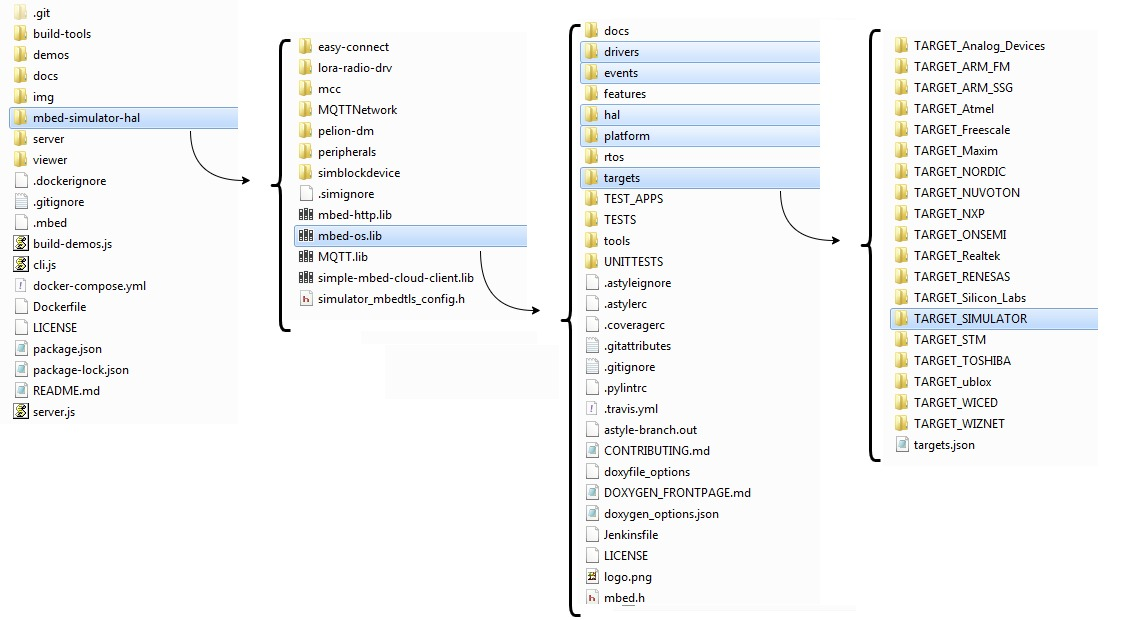
\includegraphics[scale=.35]{./Figures/estructuraMbed.jpg}
	\caption{Estructura de carpetas y archivos de \textit{Mbed Simulator}.}
	\label{fig:estructuraMbed}
\end{figure}
 
La carpeta \textquotedbl build-tools\textquotedbl contiene tres archivos javascript: 

\begin{enumerate}
	\item build-application.js, que contiene funciones para construir aplicaciones en el contexto de \textit{Mbed Simulator}. Asimismo, contiene métodos para encontrar los periféricos y manejar la construcción de componentes.
	
	\item build-libmbed.js, es un módulo de Node.js que realiza la construcción \textit{(build)} y gestión de dependencias. También, proporciona métodos que verifican las dependencias necesarias antes de la construcción.

	\item helpers.js,  es un módulo de Node.js que proporciona funciones relacionadas con operaciones de sistema de archivos, compilación, y manipulación de directorios y archivos.
\end{enumerate}
 
Dentro de la carpeta \textquotedbl demos\textquotedbl se encuentran todos los programas ejemplo que muestran cómo utilizar ciertas funcionalidades de \textit{Mbed Simulator} y son útiles como referencia para comenzar con el desarrollo en el entorno web. 
 
La carpeta \textquotedbl server\textquotedbl contiene tres archivos javascript: 

\begin{enumerate}
	\item compile.js, este archivo realiza la generación de los archivos de salida compilados a partir del codigo fuente.
	
	\item get\_ips.js, proporciona una función para la configuración de las aplicaciones de red.

	\item launch-server.js, define y configura un servidor web que permite ejecutar solicitudes de ejecución de aplicaciones, gestionar las conexiones de red y la comunicación LoRaWAN.
	
\end{enumerate}
 
La carpeta \textquotedbl viewer\textquotedbl contiene los archivos necesarios para crear interacción con el navegador. Entre estos archivos se encuentran: HTML, CSS, JavaScript, imágenes, bibliotecas de terceros o frameworks.
 
La carpeta \textquotedbl mbed-simulator-hal\textquotedbl contiene las siguiente sub-carpetas y son usadas en el contexto de \textit{Mbed Simulator}: 

\begin{itemize}
	\item easy-connect, dentro de esta carpeta se encuentran archivos que facilitan la conexión a una red utilizando Ethernet para manipular conexiones de red, sockets y eventos.
	
	\item lora-radio-drv, proporciona un marco para interactuar y controlar el módulo de radio LoRa, lo que permite enviar y recibir datos, administrar el estado y el funcionamiento.

	\item mcc, establece una cola de eventos que se utilizará para manejar eventos en \textit{Mbed Simulator}. 
	
	\item MQTTNetwork, establece la interfaz para la comunicación de red con el protocolo MQTT. 
	
	\item pelion-dm, implementación de temporizadores y manejo de eventos para la plataforma mbed.
	
	\item peripherals, proporciona implementación de los periféricos externos para ejecutarse en el entorno web.
	
	\item simblockdevice, establece una interfaz para interactuar con  dispositivos de bloques que emula un dispositivo de almacenamiento físico en el navegador web.
	
	\item mbed-os.lib, es un archivo de biblioteca en formato binario que contiene la versión del código fuente del sistema operativo de Mbed OS  para ser usada en el contexto de \textit{Mbed Simulator}.
	
\end{itemize}


Por consiguiente, la biblioteca \textquotedbl mbed-os.lib\textquotedbl contiene las siguiente carpetas: 

\begin{itemize}

	\item drivers, dentro de esa carpeta se encuentran los diversos controladores que interactúan con los periféricos de hardware dentro del contexto de \textit{Mbed Simulator}, y además, proporcionan una interfaz para acceder a ellos. 
	
	\item events, presenta archivos relacionados con la infraestructura de manejo de eventos para las tareas y operaciones de manera asíncrona.

	\item features, contiene varias subcarpetas con varios módulos que gestionan la conexión celular en dispositivos integrados, proporcionan una interfaz para interactuar con LoRaWAN, manejar la manipulación de memoria para el uso de la pila LWIP, proporciona mbed TLS, implementación del protocolo de red 6LoWPAN, sockets de red, comunicación inalámbrica de corto alcance entre dispositivos y almacenamiento de datos en sistemas embebidos. 
	
	\item hal, contiene implementaciones específicas de hardware para diferentes plataformas y microcontroladores.  
	
	\item platform, proporciona una capa de abstracción adicional sobre la capa de abstracción de hardware (HAL) .
	
	\item rtos, contiene la implementación del sistema operativo en tiempo real (RTOS).
	
	\item targets, cada sub-carpeta corresponde a un microcontrolador o una plataforma específica y, además, contiene información sobre cómo Mbed OS debe funcionar en esa plataforma en particular.
	
	\item TEST\_APPS, contiene ejemplos y aplicaciones de prueba de diferentes plataformas de hardware que se utilizan para probar y verificar diversas funcionalidades de Mbed OS.
	
	\item TESTS, contiene pruebas unitarias y de integración que verifican y validan el correcto funcionamiento de los módulos y características de Mbed OS.
	
	\item tools, contiene herramientas y utilidades para el desarrollo, compilación, depuración y prueba para diferentes plataformas de hardware y sistemas operativos.

	\item UNITTESTS, contiene pruebas unitarias para diferentes componentes del sistema operativo Mbed.

	\item mbed.h, dentro del contexto de \textit{Mbed Simulator} contiene declaraciones y definiciones iniciales para que estén disponibles para el desarrollo web del usuario. 
	
\end{itemize}


Después, al eliminar módulos y dependencias innecesarias, tales como: mbed-http, simple-mbed-cloud-client, features, rtos y todas las sub-carpetas dentro de la carpeta \textquotedbl target\textquotedbl excluyendo a la sub-carpeta TARGET\_SIMULATOR.
Luego, se procedió a evaluar la compatibilidad de su arquitectura. Durante el proceso, en primer lugar, se analizó si la arquitectura proporcionaba funcionalidades para la interacción con los usuarios. Incluso, de adaptarse fácilmente a futuros desarrollos y cambios, permitiendo un crecimiento escalable.

Además, la mantenibilidad y flexibilidad también fueron aspectos evaluados. Otro punto esencial, fueron las tecnologías y herramientas utilizadas, lo cual implicó una curva de aprendizaje adicional. 

Actualmente, \textit{Mbed Simulator} presenta las siguientes limitaciones:

\begin{enumerate}
	\item Dentro de un bucle infinito \texttt{while(1)}, es necesario agregar un retraso \newline(\texttt{delay)}, de lo contrario, el navegador no puede actualizar la interfaz de la plataforma web ni responder a eventos del usuario. Esto significa que el navegador no tiene la oportunidad de realizar otras tareas o responder a eventos mientras el bucle está en ejecución. Como resultado, el navegador se bloquea o congela y puede dejar de responder.
	
	\item En cada iteracion, la ejecución del programa puede variar en términos de tiempo, lo que puede afectar a la precisión en la sincronización de eventos dentro de la aplicación.

	\item En \textit{Mbed Simulator}, no hay restricciones significativas en cuanto a cuánta memoria se puede asignar al stack o al heap  de un programa, lo cual difiere del hardware físico, donde sí existen limitaciones de memoria.
	
	\item Dentro del entorno web, las interrupciones no se manejan de la misma manera que en un sistema embebido real, debido a que no tienen prioridad o no afectan la ejecución del programa principal.
	
	\item Sin RTOS. No tiene la capacidad de ejecutar múltiples hilos de manera concurrente como lo haría un RTOS. Todo el código se ejecuta en un solo hilo. Se puede utilizar la biblioteca mbed-events para manejar ciertos aspectos de concurrencia, usando eventos y temporizadores.

\end{enumerate}

Finalmente, una vez confirmada su compatibilidad para los propósitos del presente trabajo, se tomó la decisión de seleccionarlo y empezar el desarrollo.


\section{Arquitectura de la plataforma web}

Después del análisis de \textit{Mbed Simulator}, se modificaron los nombres de las carpetas y archivos de configuración para adaptarlos al entorno del emulador EDU-CIAA. Luego, se reemplazó \textquotedbl mbed-os\textquotedbl por la biblioteca \textit{\textbf{sAPI}}, pero se mantuvieron algunos componentes propios de Mbed, como \textquotedbl events\textquotedbl y \textquotedbl callback\textquotedbl, para agilizar el desarrollo.
  
En la figura \ref{fig:estructuraCiaa} se exhibe la estructura de las carpetas y archivos del  \textit{Emulador de la placa EDU-CIAA}.

\begin{figure}[ht]
	\centering
	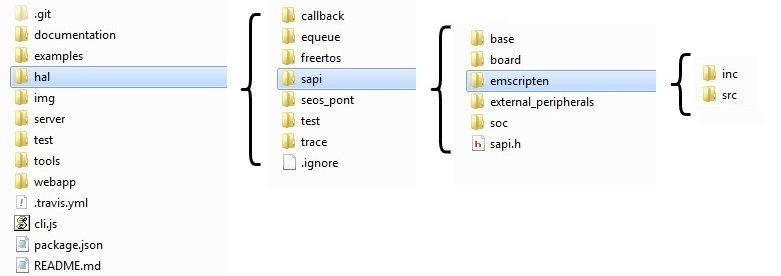
\includegraphics[scale=.50]{./Figures/estructuraCiaa.jpg}
	\caption{Estructura de carpetas y archivos de \textit{Mbed Simulator}.}
	\label{fig:estructuraCiaa}
\end{figure}
 

La emulación a nivel de API proporciona una capa de abstracción para el entorno de desarrollo del usuario, de modo que permite escribir aplicaciones en \textit{C} y ejecutarlas en la plataforma de emulación. 

Al utilizar esta capa de abstracción, se pudo replicar las funcionalidades y las características de configuración de la biblioteca \textit{\textbf{sAPI}} en un entorno diferente, en este caso, en un entorno web.


En el diagrama de bloques de la figura \ref{fig:Arquitectura} se muestra la arquitectura básica de una aplicación de usuario que ejecuta el emulador de la placa EDU-CIAA-NXP.


\begin{figure}[ht]
	\centering
	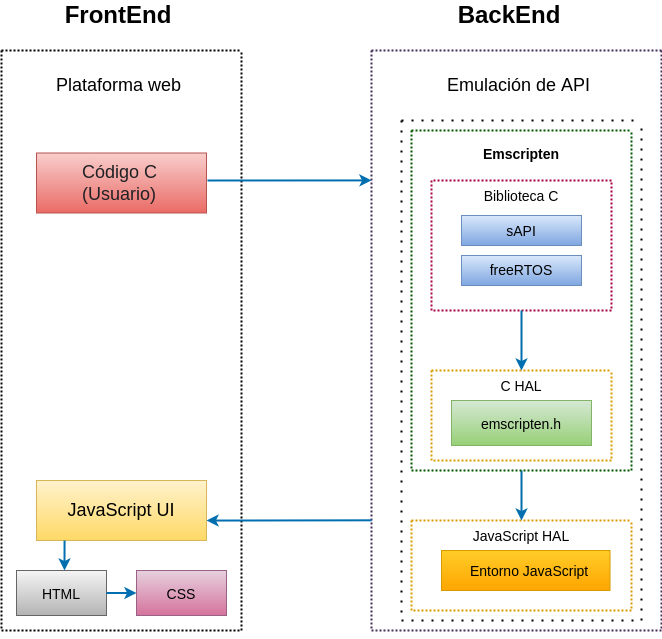
\includegraphics[scale=.55]{./Figures/Arquitectura.png}
	\caption{Diagrama de bloques arquitectura de la plataforma.}
	\label{fig:Arquitectura}
\end{figure}

A continuación, se presenta una breve descripción de cada componente del diagrama de bloques de la figura \ref{fig:Arquitectura}:

\begin{enumerate}
	\item El usuario escribe un programa en código de lenguaje \textit{C}, que utiliza la biblioteca \textit{\textbf{sAPI}} u otras. 
	
	\item El código del usuario se conecta a través de la plataforma de emulación con la capa 
\textit{Biblioteca C} que proporciona la emulación a nivel de API, de la biblioteca \textit{\textbf{sAPI}}.
	
	\item La capa \textit{Biblioteca C} se comunica con la capa \textit{C HAL} (capa abstracción de hardware) escrita en \textit{C}. Esta capa \textit{C HAL} proporciona las definiciones necesarias para que el compilador de \textit{Emscripten} traduzca el código escrito en lenguaje \textit{C} a código que puede ser ejecutado en el entorno web.
	
	\item La capa \textit{JavaScript HAL} se comunica con la capa \textit{C HAL}  a través de los archivos \textit{WebAssembly} y \textit{JavaScript} generados por el proceso de compilación de \textit{Emscripten}.
	
	\item La capa de abstracción de JavaScript (\textit{JavaScript HAL}) actúa como intermediario entre las capa \textit{C HAL} y la interfaz de usuario en \textit{JavaScript} (\textit{JavaScript UI}). Y además, se encarga de distribuir eventos y llamadas entre ambas capas.
	
\item La interfaz de usuario en \textit{JavaScript} (\textit{JavaScript UI}) maneja los eventos procedentes de la capa \textit{JavaScript HAL}. No interactúa directamente con el código \textit{JavaScript} y \textit{WebAssembly} resultante del código \textit{C}.

\item La capa \textit{JavaScript UI} accede y modifica dinámicamente los elementos HTML, que utilizan reglas de estilo \textit{CSS} para la presentación en la plataforma web.
	
\end{enumerate}


En resumen, el diagrama representa cómo un programa escrito en lenguaje \textit{C} interactúa con la capa de abstracción de la emulación a nivel de API hasta llegar a la interfaz de usuario en \textit{JavaScript}. La compilación con \textit{Emscripten} permite que el código en \textit{C} se ejecute en el navegador web, lo que posibilita la ejecución del programa de usuario en un entorno basado en la web.


\section{Frontend}
En esta parte de la plataforma web se implementó el desarrollo de la interacción entre el \textit{backend} y el navegador del usuario.


\subsection{Diseño de la Interfaz de Usuario}

Para el desarrollo de la interfaz, se optó por un diseño intuitivo, de manera que el usuario se sienta familiarizado con las herramientas de trabajo y que la disposición de los componentes sea cómoda y esté organizada al momento de usarlas.

La figura \ref{fig:PlataformaEmulador1} muestra la plataforma web del Emulador de la placa EDU-CIAA-NXP.

\begin{figure}[ht]
	\centering
	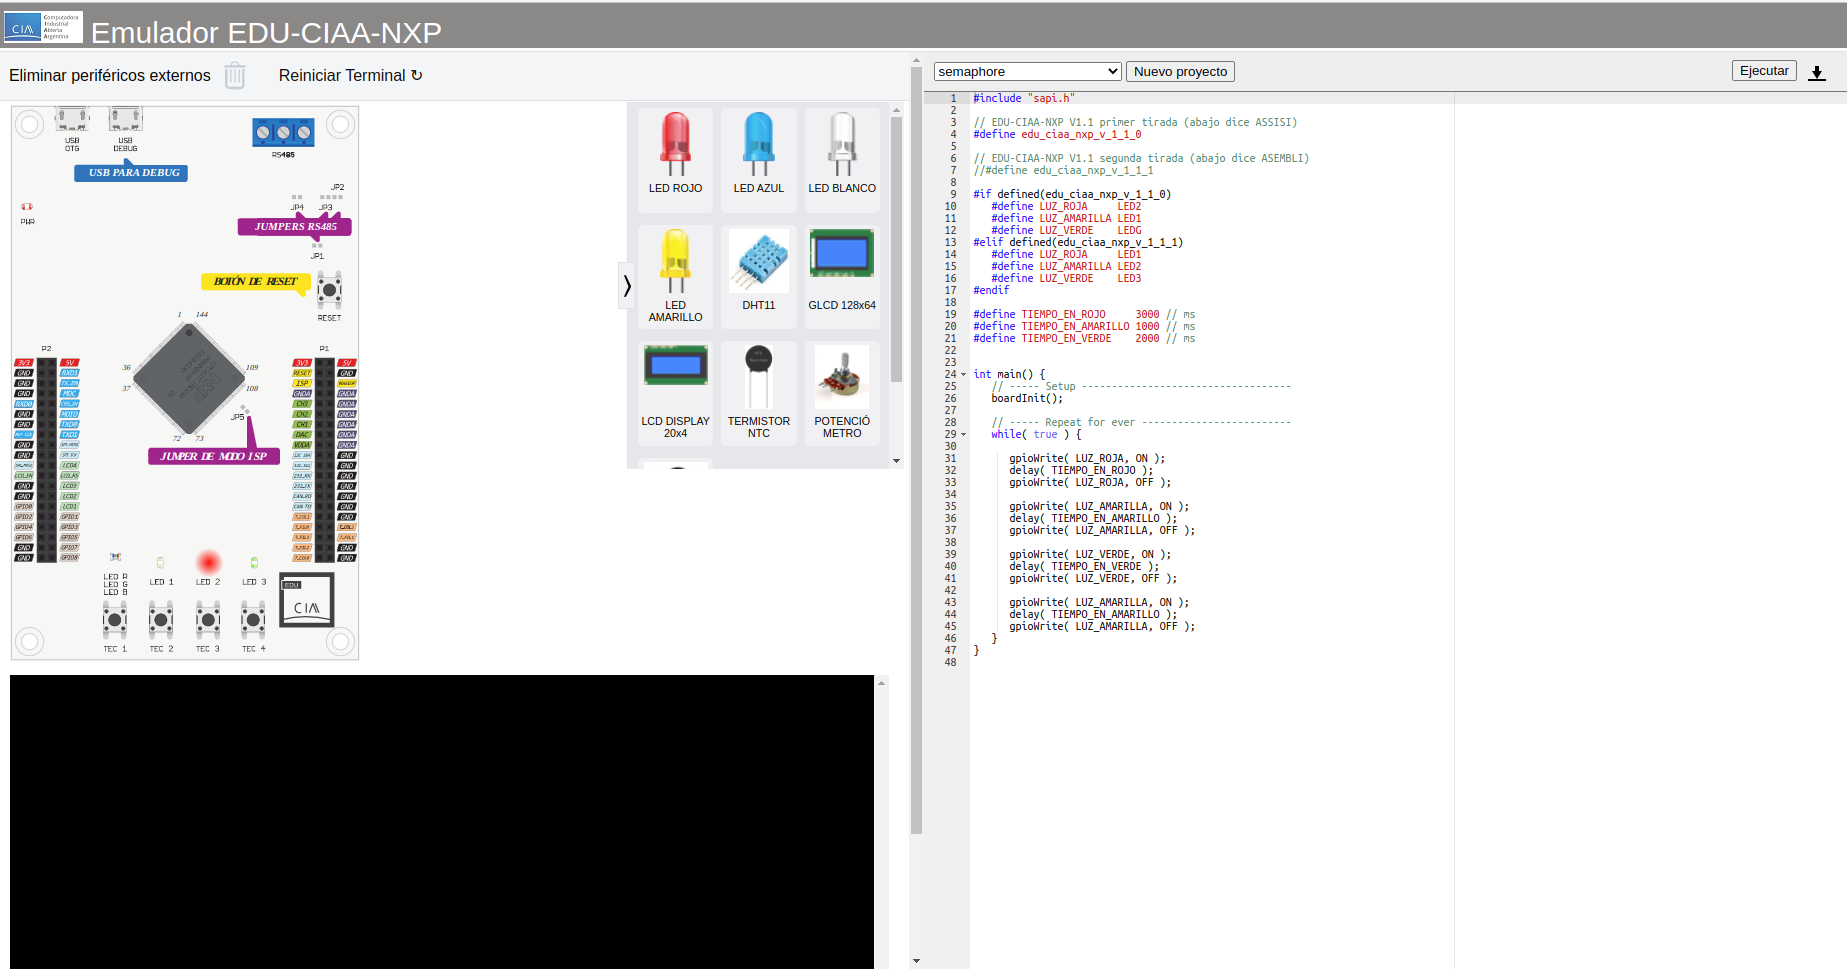
\includegraphics[scale=.27]{./Figures/PlataformaEmulador.png}
	\caption{Plataforma de emulación para la placa EDU-CIAA-NXP.}
	\label{fig:PlataformaEmulador1}
\end{figure}


Para su estudio, dividimos la plataforma web en tres partes. En la figura \ref{fig:PlataformaEmulador2}, se muestra la parte izquierda y superior de la interfaz gráfica para interactuar con el hardware. La figura \ref{fig:PlataformaEmulador3} muestra la parte inferior izquierda, donde se visualiza la salida de la consola. Finalmente, en la figura \ref{fig:PlataformaEmulador4}, se muestra la parte derecha de la interfaz gráfica destinada a la aplicación de usuario.

\begin{figure}[ht]
	\centering
	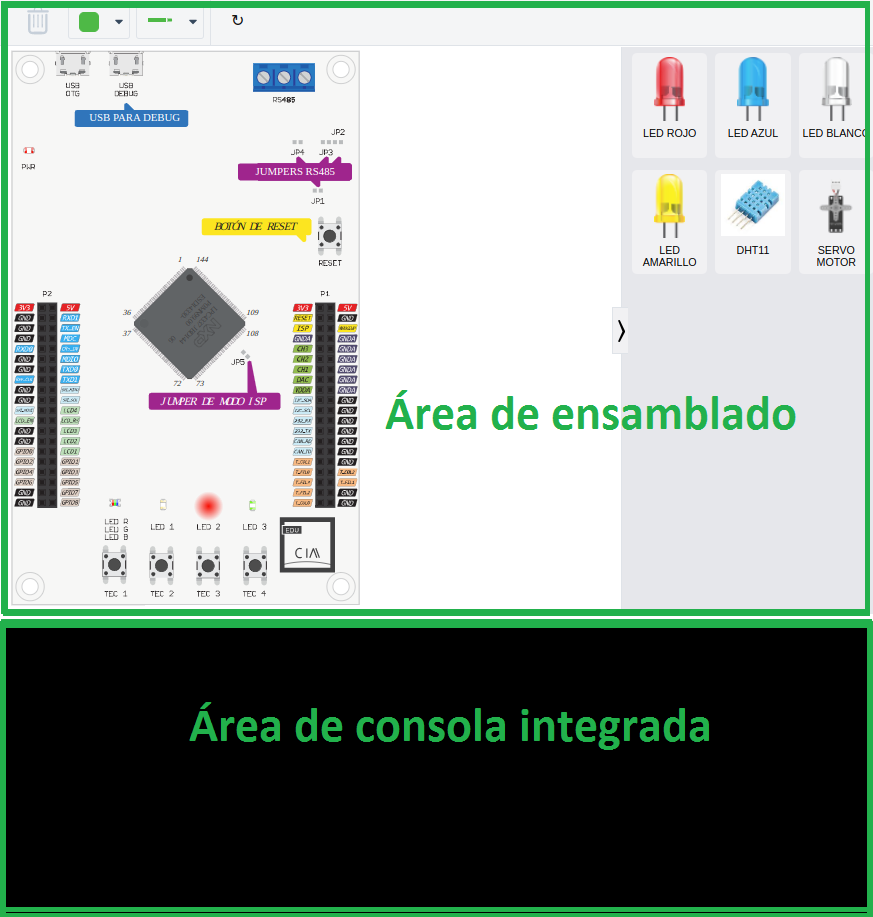
\includegraphics[scale=.57]{./Figures/PlataformaEmulador1.png}
	\caption{parte izquierda y superior de la plataforma de emulación de la placa EDU-CIAA-NXP.}
	\label{fig:PlataformaEmulador2}
\end{figure}


\begin{figure}[ht]
	\centering
	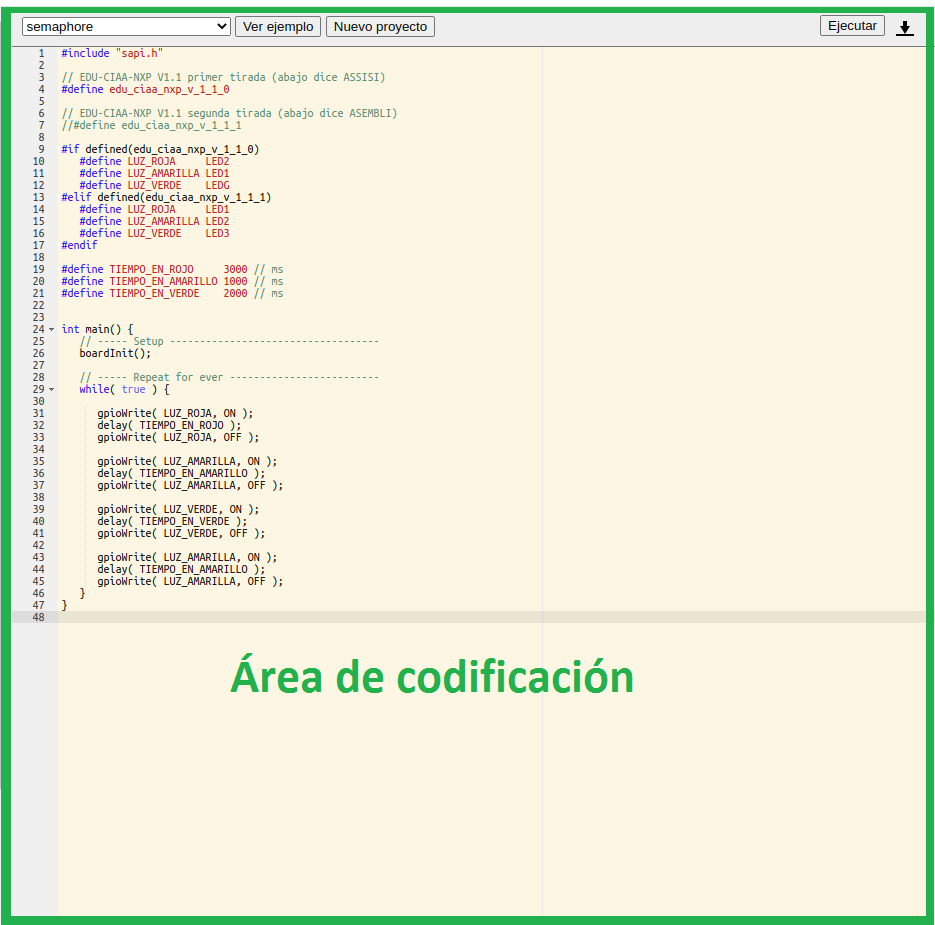
\includegraphics[scale=.58]{./Figures/PlataformaEmulador2.png}
	\caption{Parte inferior izquierda de la plataforma de emulación de la placa EDU-CIAA-NXP.}
	\label{fig:PlataformaEmulador3}
\end{figure}


\hfill \break
\hfill \break
\hfill \break
\hfill \break
\hfill \break
\hfill \break
\hfill \break

\begin{figure}[ht]
	\centering
	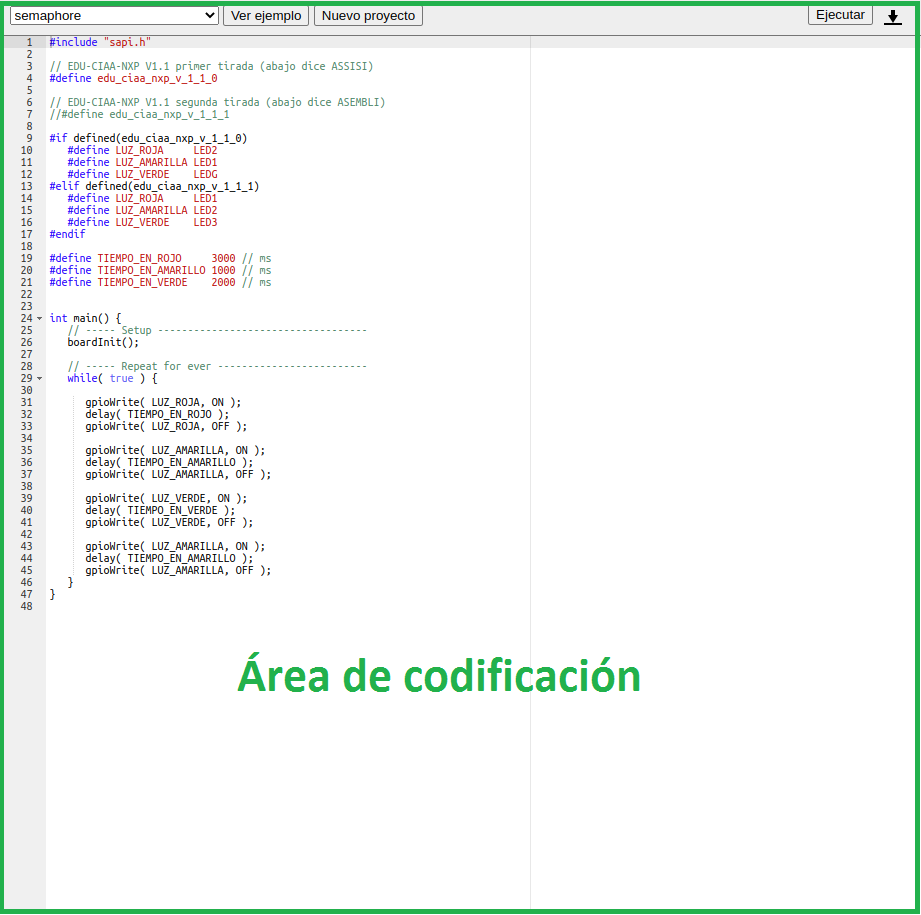
\includegraphics[scale=.45]{./Figures/PlataformaEmulador3.png}
	\caption{Parte derecha de la plataforma de emulación de la placa EDU-CIAA-NXP.}
	\label{fig:PlataformaEmulador4}
\end{figure}

Por consiguiente, el diseño de la interfaz de usuario de la plataforma proporciona las siguientes áreas:

\begin{itemize}
	\item Área de ensamblado: el valor predeterminado muestra la placa EDU-CIAA-NXP, y también se permite agregar componentes.
	\item Área de codificación: se proporciona un editor de código en línea para programar con la placa EDU-CIAA-NXP. La primera vez que se accede a la platafoma se muestra en ejecución un ejemplo de código predeterminado.
	\item Área de consola integrada: se muestra en una ventana la salida que se vería a través del puerto serie. 
\end{itemize}


Debido a las áreas de trabajo que presenta la plataforma, el
usuario programador podrá realizar las siguientes tareas:

\begin{itemize}
	\item Ver los programas de ejemplo predeterminados.
	\item Crear un nuevo proyecto.
	\item Ejecutar un programa de ejemplo o uno nuevo.
	\item Editar programas.
	\item Visualizar los cambios programados para la placa virtual.
	\item Agregar nuevos componentes.
	\item Ver los errores obtenidos en la programación.
	\item Ver lo programado en la salida de consola.
\end{itemize}

\subsubsection{Área de ensamblado}

Para el desarrollo de la placa EDU-CIAA-NXP Y componentes externos se usaron dibujos en formato de gráficos vectoriales bidimensionales (SVG) por las siguientes características:

\begin{itemize}
	\item Son más ligeras, entonces se cargan más rápido en el navegador.
    \item Por su capacidad de ser modificado por medio de \textit{JavaScript}. Por lo tanto, se pudieron crear imágenes interactivas.
	\item Evitan que las imagenes se deformen y no pierden calidad.
	\item Permite programar animaciones.
\end{itemize}

En ese sentido, para la capa de programación \textit{JavaScript UI}, se pudo implementar el comportamiento interactivo para los botones de la placa (TEC1, TEC2, TEC3 y TEC4) usando el código SVG generado para la placa EDU-CIAA-NXP, incluso, se pudo modificar también el comportamiento de los LEDs, que permitió mostrar dinamicamente en la placa el encendido y apagado.

Además, con el objetivo de optimizar la experiencia del usuario, esta área permite elegir uno o más dispositivos virtuales de entrada/salida desde la barra lateral \textit{sidebars} derecho, dentro de la barra se exhiben todos los perifericos disponibles en la plataforma web. 

Una vez que el usuario elige un periférico de la barra lateral y realiza la configuración de las conexiones, la barra automáticamente colapsa, ocultándose del área de ensamblado. Al colapsarse, se muestra el periférico integrado en la aplicación. Asimismo,  el usuario tiene la opción de volver a expandir la barra lateral para agregar un nuevo periférico.


En la figura \ref{fig:AgregarPeriferico} se observa que el usuario puede elegir qué componente agregar a la aplicación y en la figura \ref{fig:AgregarPeriferico2} se muestra que el componente se agregó a la aplicación.
\hfill \break
\hfill \break
\hfill \break
\hfill \break
\hfill \break
\hfill \break
\hfill \break
\hfill \break
\hfill \break
\hfill \break
\hfill \break
\hfill \break
\hfill \break
\hfill \break
\hfill \break
\hfill \break
\hfill \break

\begin{figure}[ht]
	\centering
	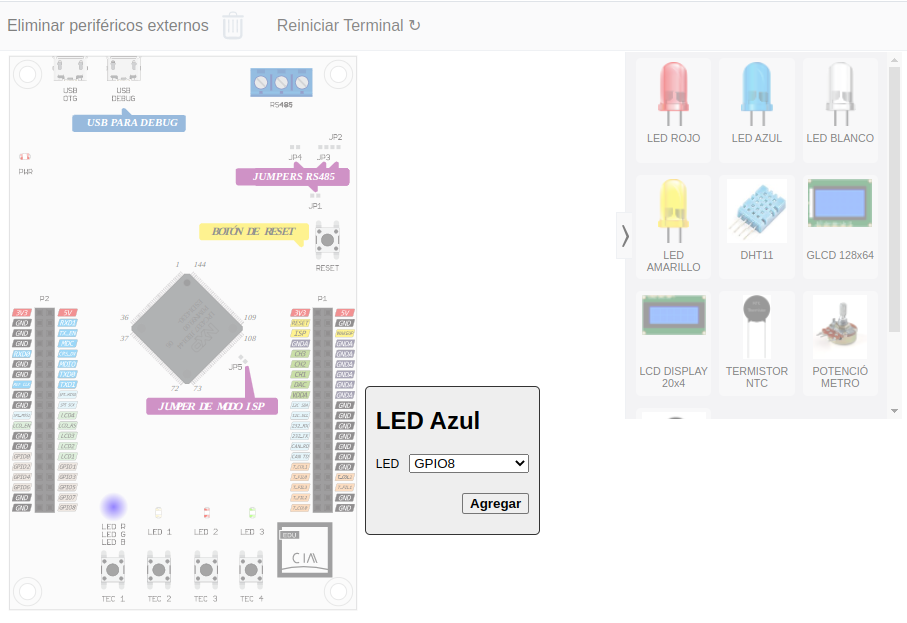
\includegraphics[scale=.41]{./Figures/AgregarPeriferico.png}
	\caption{Agregar periférico.}
	\label{fig:AgregarPeriferico}
\end{figure}


\begin{figure}[ht]
	\centering
	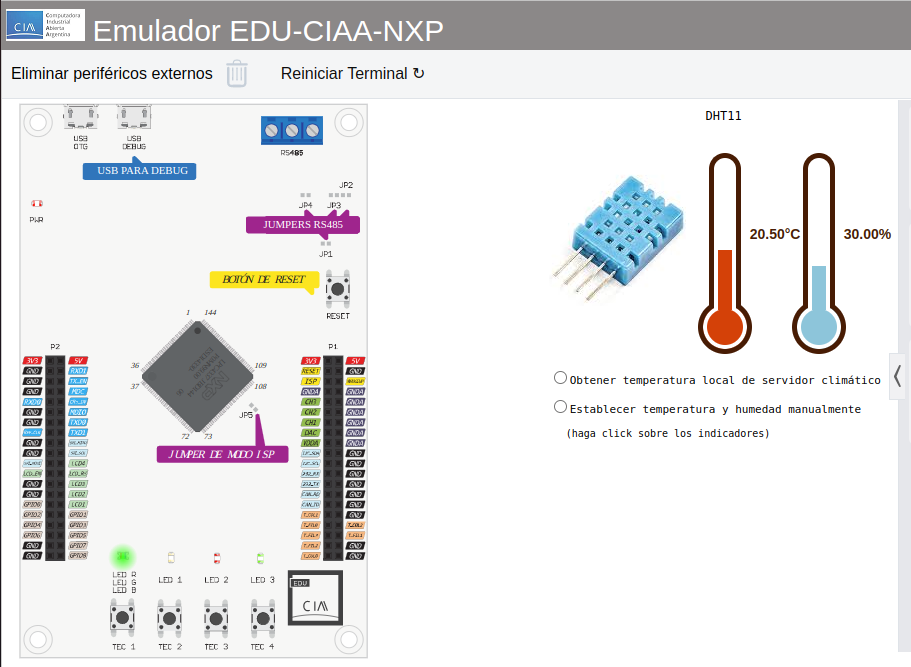
\includegraphics[scale=.41]{./Figures/AgregarPeriferico2.png}
	\caption{Periférico agregado en el área de ensamblado. }
	\label{fig:AgregarPeriferico2}
\end{figure}


\subsubsection{Área de codificación}

Esta parte de la plataforma se reserva al usuario para que pueda programar sus propias aplicaciones. Esta ventana de edición presenta las siguientes capacidades:

\begin{itemize}
\item Manejar la sintaxis para el lenguaje C.
\item Soportar el uso de las constantes, como por ejemplo: '\#define'.
\item Permitir el uso de las palabras claves, comentarios, etc.
\item Permitir el resaltado de líneas de código, sangría automática y número de línea.
\item Utilizar la función buscar (ctrl + f).
\item Utilizar la función buscar/reemplazar (ctrl + h).
\item Utilizar la función rehacer (ctrl + y).
\end{itemize}


Para compilar un programa, la plataforma provee al usuario el botón “ejecutar”. Sin embargo, si hubo problemas de sintaxis, errores lógicos, etc., se mostrarán esos errores al usuario.

En la figura \ref{fig:PlataformaErrores2} se muestra el código que generó los errores de compilación y en la figura \ref{fig:PlataformaErrores1} se observa los errores de compilación en el área de ensamblado.



\begin{figure}[ht]
	\centering
	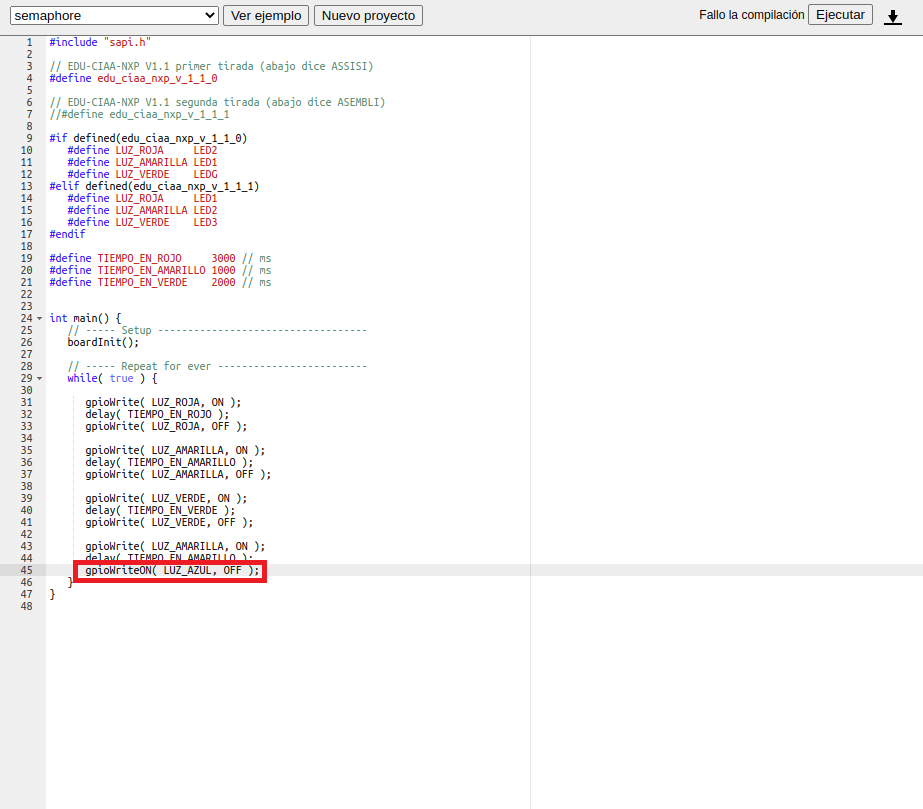
\includegraphics[scale=.46]{./Figures/PlataformaErrores1.png}
	\caption{Código que generó los errores de compilación.}
	\label{fig:PlataformaErrores2}
\end{figure}



\begin{figure}[ht]
	\centering
	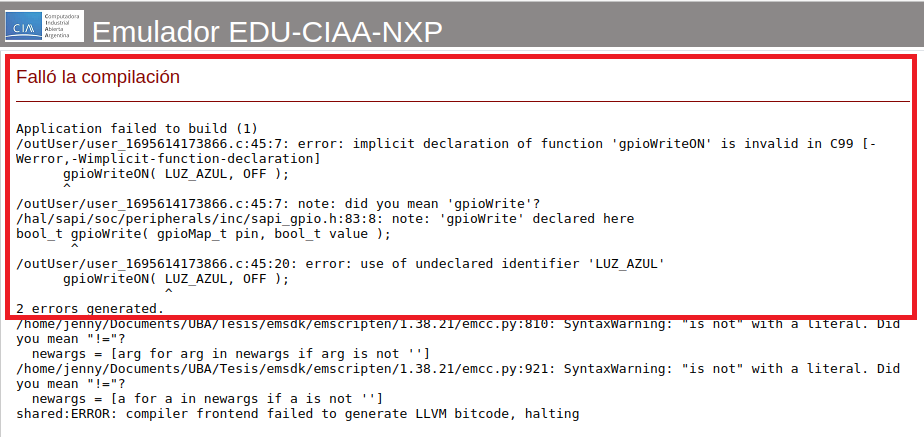
\includegraphics[scale=.46]{./Figures/PlataformaErrores2.png}
	\caption{Errores de compilación.}
	\label{fig:PlataformaErrores1}
\end{figure}

También se implementó una estructura jerárquica en la lista desplegable de ejemplos. El propósito es organizar y presentar los ejemplos agrupados por periféricos, de manera más ordenada y fácil de navegar para el usuario.

La figura \ref{fig:listExamples} muestra la estructura jerárquica en la lista.

\begin{figure}[ht]
	\centering
	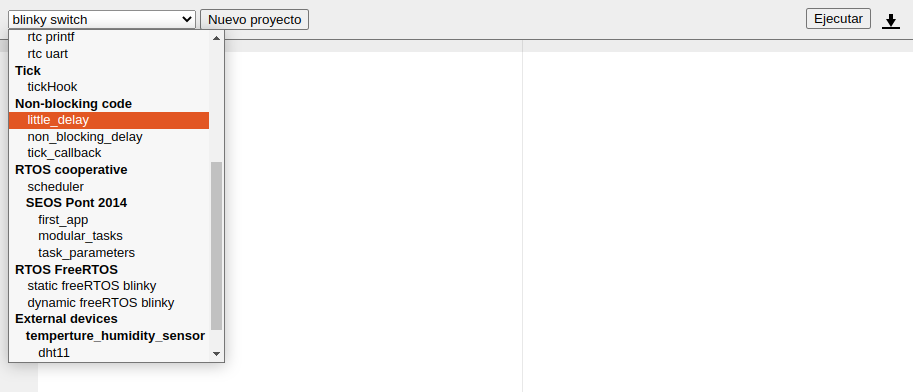
\includegraphics[scale=.25]{./Figures/listExamples.jpg}
	\caption{Estructura jerárquica de ejemplos. }
	\label{fig:listExamples}
\end{figure}

Ademas, al seleccionar algún ejemplo para un periférico externo de la lista desplegable, automáticamente se cargara dentro del área de ensamblado el periférico con las conexiones a los pines configuradas por defecto.

La figura \ref{fig:cargarPeriferico} muestra el periférico agregado al seleccionar el ejemplo \textquotedbl joystick\textquotedbl.

\begin{figure}[ht]
	\centering
	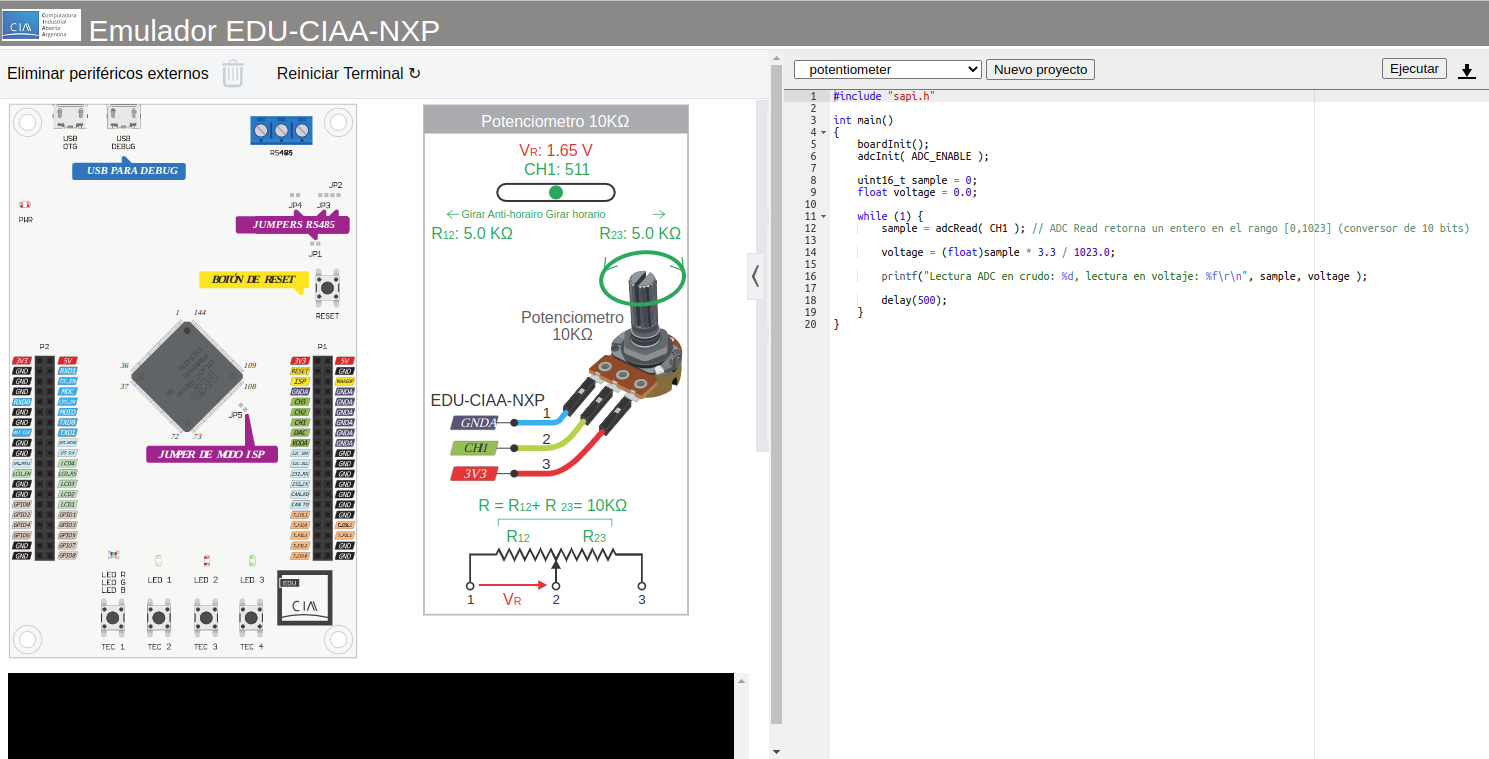
\includegraphics[scale=.20]{./Figures/cargarPeriferico.png}
	\caption{Carga automática de Periférico. }
	\label{fig:cargarPeriferico}
\end{figure}



\subsubsection{Área de consola integrada}

Dentro del código traducido en el proceso de compilación por \textit{Emscripten}, se encuentran las siguientes funciones definidas y configuradas previamente, las cuales son: 

\begin{itemize}
\item \texttt{print}, esta función envía el texto a la terminal de la interfaz gráfica del emulador web, al utilizar la función \texttt{terminal.write}.
\item \texttt{printErr}, se comunica con la consola de error del navegador, al usar \newline \texttt{console.error}.
\end{itemize}

Ambas funciones interactuan con el código \textit{JavaScript}. La función \texttt{printErr} se comunica con la consola de error del navegador y la función \texttt{print} se comunica con la terminal del emulador web a través de la biblioteca xterm.js, que es un componente de terminal de front-end escrito en \textit{JavaScript} y que permite construir terminales en el navegador. 

Entre las principales características de xterm.js se destaca:

\begin{itemize}
	\item Funciona con la mayoría de las aplicaciones de terminal, como bash, es compatible con aplicaciones basadas y eventos de mouse.
	\item Es de alto rendimiento, por eso es realmente rápido.
	\item No requiere de dependencias externas para funcionar, sin embargo, la dependencia principal para el funcionamiento básico es el propio navegador web.
	\item API bien documentada.
\end{itemize}


Además de las características de Xterm.js, esta biblioteca de \textit{JavaScript} es usado por varios proyectos populares como VS Code, Hyper y Theia que lo usan, de ahí que, el soporte en la comunidad de desarrolladores es amplio.

En la figura \ref{fig:Terminal1} se muestra un programa de usuario que generó la salida por consola.

\begin{figure}[ht]
	\centering
	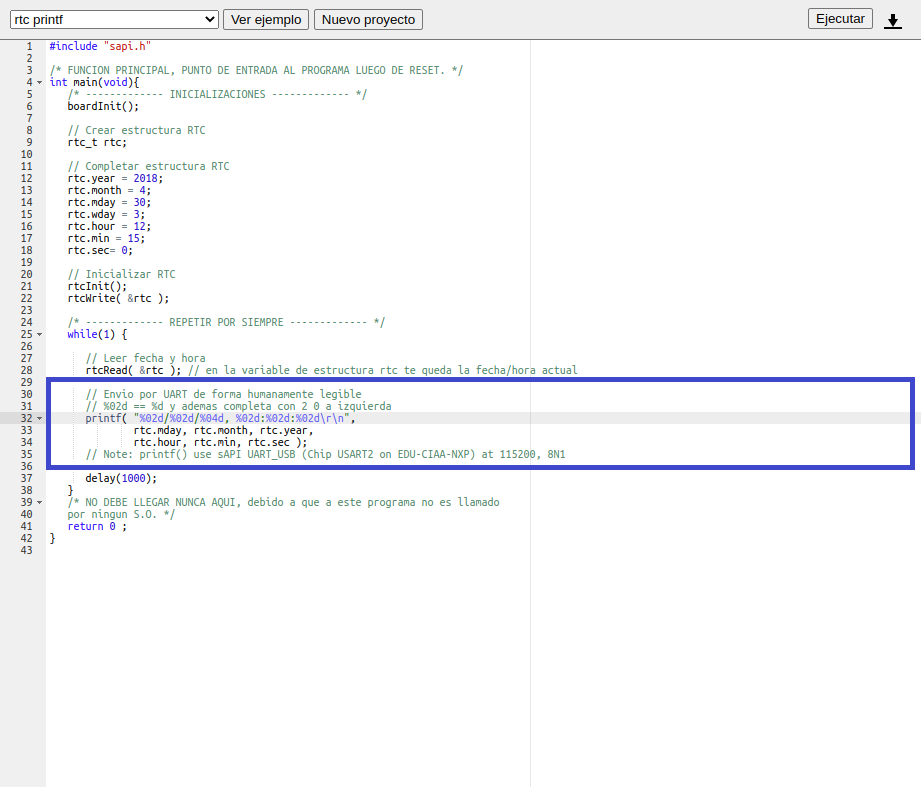
\includegraphics[scale=.41]{./Figures/Terminal1.png}
	\caption{Programa de usuario.}
	\label{fig:Terminal1}
\end{figure}
 


En la figura \ref{fig:Terminal2} se puede observar la salida por consola.

\begin{figure}[ht]
	\centering
	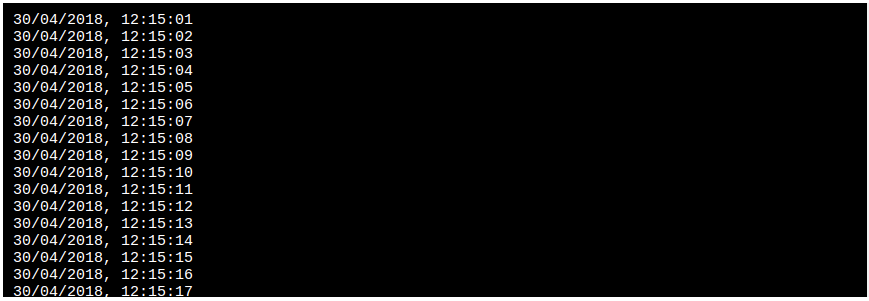
\includegraphics[scale=.45]{./Figures/Terminal2.png}
	\caption{Salida de la terminal serie.}
	\label{fig:Terminal2}
\end{figure}
 
 
 \hfill \break
\hfill \break
\hfill \break
\hfill \break
\hfill \break

\subsection{JavaScript UI}

Esta capa se desarrolló con el propósito de que se comunique con la capa \textit{JavaScript HAL}, y también con el objetivo de proporcionar componentes de código, utilidades y manejo de eventos en la aplicación de usuario.

Por tanto, para lograr la comunicación con la capa \textit{JavaScript HAL}, se desarrolló en esta capa los objetos que se sucriben al detector de eventos programados en la \textit{HAL}.

\textit{JavaScript} permite crear oyentes, utilizando el método \texttt{on()} y pasando como argumento el nombre del evento al que se quiere suscribir. De esta manera, se  programaron varios subscriptores para un mismo evento en diferentes archivos \textit{JavaScript} dentro de esta capa. En consecuencia, se logró una mayor interactividad entre los componentes de la plataforma.

Es decir, cuando se emite algún evento en la \textit{HAL}, entonces el oyente suscrito a ese evento en esta capa \textit{UI} lo podrá escuchar y realizar las acciones que correspondan para la funcionalidad requerida. La figura \ref{fig:EventemitterNodeJSUI} describe esta situación.


\begin{figure}[ht]
	\centering
	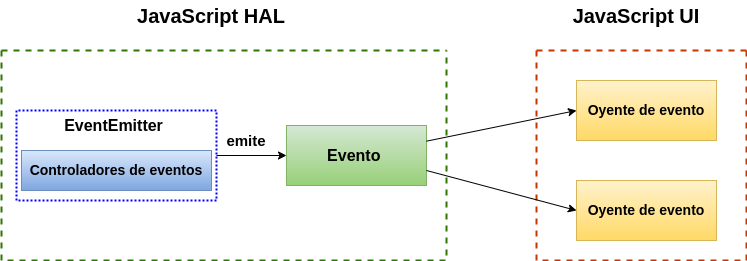
\includegraphics[scale=.51]{./Figures/EventemitterNodeJSUI.png}
	\caption{Diagrama de bloques de los oyentes de \textit{EventEmitter} en la capa UI.}
	\label{fig:EventemitterNodeJSUI}
\end{figure}




\subsection{Aplicación de Usuario}
La plataforma de emulación para la placa EDU-CIAA-NXP es una aplicación en línea, que se ejecuta en el \textit{browser} del usuario. La interfaz fue diseñada como una herramienta que permite al usuario realizar sus tareas de programación dentro de una plataforma simple e intuitiva.

Sin embargo, existen algunas limitaciones que se deben tener en cuenta.

\begin{itemize}
	\item Las unidades de tiempo especificadas por los valores en las constantes, por ejemplo cuando el usuario define \texttt{TASK1\_PERIODICITY} con un valor de 1000 para ser usado dentro del codigo siguiente: 
	
\begin{lstlisting}[caption={Ejemplo TASK1\_PERIODICITY}]
#define TASK1_PERIODICITY 1000} 

if( task1Counter++ == TASK1_PERIODICITY ){
  task1();
  task1Counter = 0;
}
\end{lstlisting}	
	


Significa que la tarea  planificada se ejecutará cada 1000 milisegundos en la placa fisica. Sin embargo, en el emulador web, la velocidad de ejecución puede variar y no necesariamente coincidir con el tiempo real. Por lo tanto, el tiempo de ejecución de cada iteración de la tarea \texttt{task1} podría ser más lento en el emulador web. Estas diferencias en la ejecución se deben a las limitaciones inherentes de \textit{JavaScript} y \textit{Emscripten}, que pueden afectar la precisión del tiempo.

\end{itemize}

\section{Backend}

En esta capa de programación se desarrolló toda la lógica necesaria para emular las funcionalidades que proporcionan las bibliotecas: \textit{\textbf{sAPI}}, \textit{\textbf{freertos}} y \textit{\textbf{seos\textunderscore pont}} para la placa EDU-CIAA-NXP.

\subsection{Biblioteca C}

En primer lugar, se identificaron las funciones de las bibliotecas \textit{C} originales para empezar a emular. Luego, en el emulador se crearon interfaces que reflejen las estructuras de las bibliotecas originales, que incluyo definiciones de funciones, estructuras de datos y constantes.

Es decir, en las funciones originales se examinaron los parámetros de entrada y los valores de retorno, para luego mapearlos correctamente en las definiciones de las funciones del emulador.  A modo de referencia se muestra en la tabla \ref{tab:gpioMap} las definiciones de las funciones para \texttt{sapi\_gpio.h}, que incluye los nombres de la funciones, los tipos de parámetros y el tipo de valor de retorno. Cabe destacar que estas definiciones son idénticas tanto en las \textit{\textbf{sAPI}} como en el emulador, lo que permite una fácil correspondencia entre ambas.

\begin{table}[h]
	\centering
	\caption[Módulo \textit{GPIO}]{Módulo \textit{GPIO}}
	\begin{tabular}{l c c}    
		\toprule
		\textbf{Nombre de la función} 	 & \textbf{Parámetros} 		& \textbf{Tipo de retorno}  \\
		\midrule
		gpioInit & gpioMap\_t, gpioInit				&  bool\_t \\		
		gpioRead	 & gpioMap\_t				&  bool\_t \\
		gpioWrite	 & gpioMap\_t, bool\_t				&  bool\_t \\
		gpioToggle	 & gpioMap\_t				&  bool\_t \\
		\bottomrule
		\hline
	\end{tabular}
	\label{tab:gpioMap}
\end{table}



Al igual que en la biblioteca \textit{\textbf{sAPI}} del proyecto CIAA, los archivos de código fuente para la plataforma de emulación, conservan el mismo nombre, por ejemplo  \texttt{sapi\_gpio.c}. Sin embargo, la implementación de las funciones es totalmente distinta. En el caso de la biblioteca \textit{\textbf{sAPI}} del proyecto CIAA, para \texttt{sapi\_gpio.c}  se incluyen los archivos de encabezado: \texttt{gpio\_18xx\_43xx.h} y \newline \texttt{scu\_18xx\_43xx.h}. Y en el caso de la plataforma de emulación se usa otro archivos de encabezado como \texttt{gpio\_api.h} para replicar el mismo comportamiento.

A continuación, se presenta una comparación entre las clases del módulo GPIO de la biblioteca \textit{\textbf{sAPI}} del proyecto CIAA y el módulo GPIO implementado en la plataforma de emulación. 

La figura \ref{fig:GPIOsAPI} muestra las dependencias que se usan para la implementación de \newline \texttt{sapi\_gpio.c} del proyecto CIAA y en la figura \ref{fig:GPIOEmulador} se muestran las dependencias utilizadas en el emulador para el mismo módulo, logrando el \textit{port} al emulador de las funciones para el manejo del periférico GPIO.




\begin{figure}[ht]
	\centering
	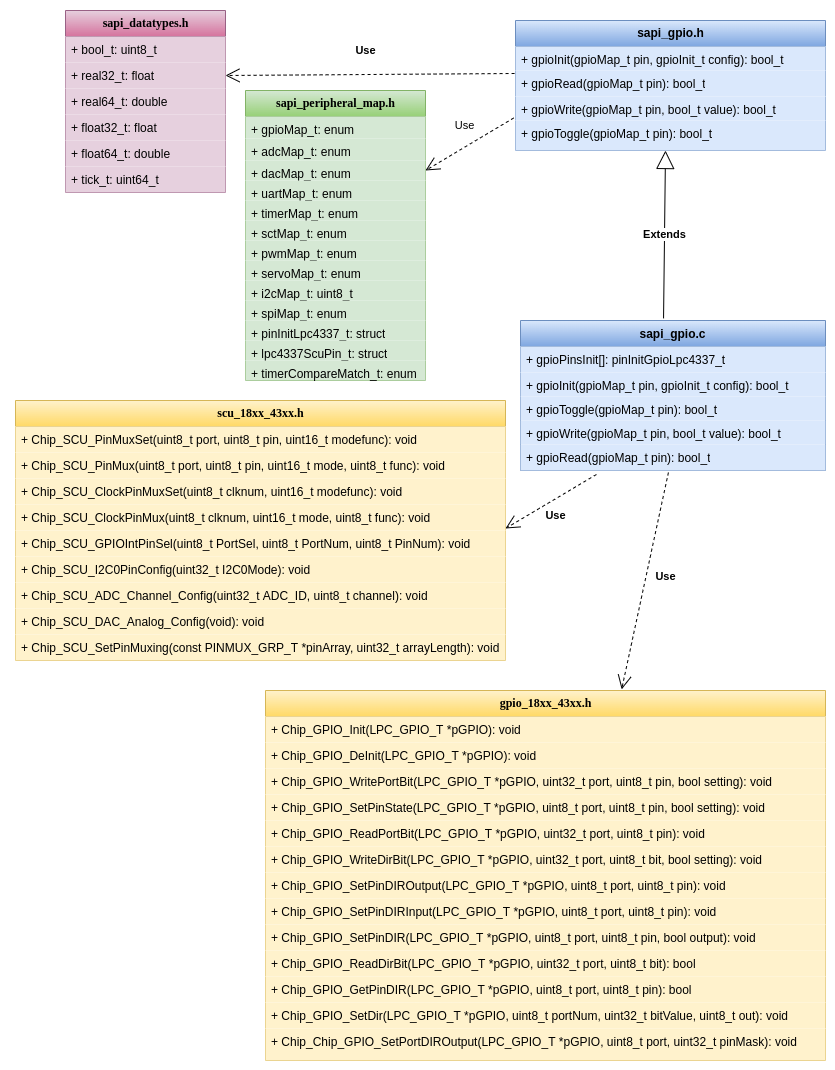
\includegraphics[scale=.41]{./Figures/DiagramaClasesGPIOsAPI.png}
	\caption{Diagrama de dependencias del módulo \textit{GPIO} de la biblioteca \textit{\textbf{sAPI}} del proyecto CIAA.}
	\label{fig:GPIOsAPI}
\end{figure}


\hfill \break
\hfill \break


\begin{figure}[ht]
	\centering
	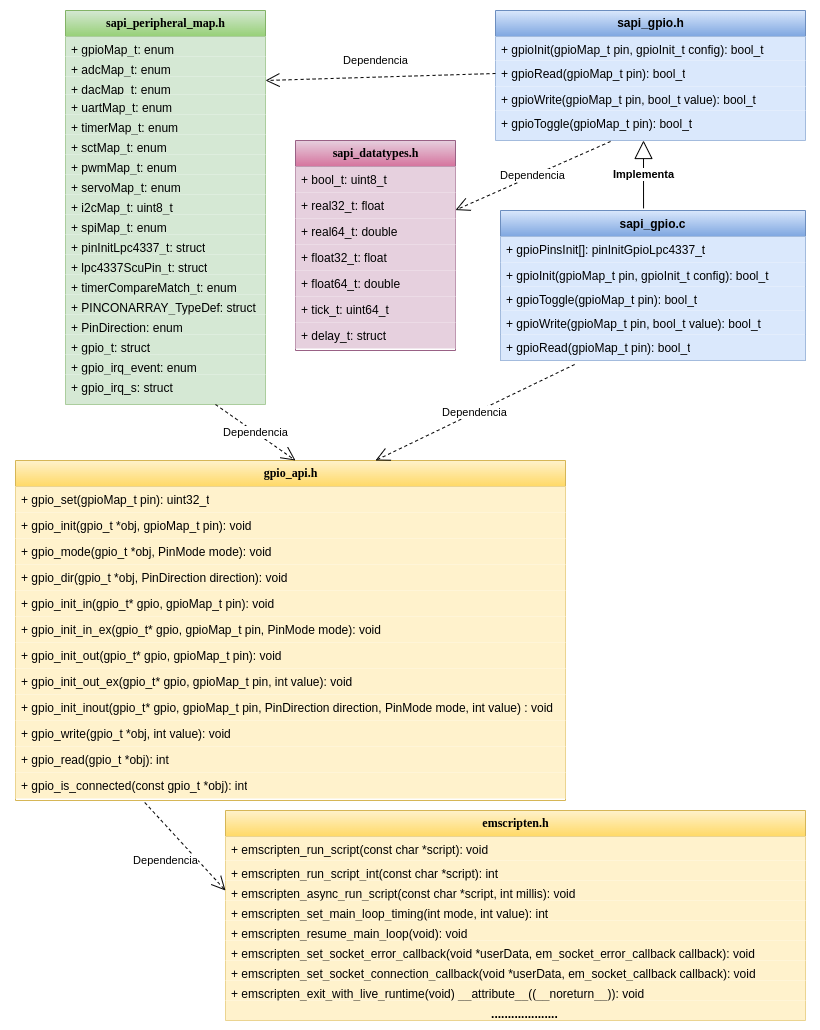
\includegraphics[scale=.41]{./Figures/DiagramaClasesEmulador.png}
	\caption{Diagrama de dependencias del módulo \textit{GPIO} de la plataforma de emulación para la placa EDU-CIAA-NXP.}
	\label{fig:GPIOEmulador}
\end{figure}


Para todos los demás módulos de la biblioteca \textit{\textbf{sAPI}} para la pogramación de periféricos del microcontrolador se siguió esta misma lógica. Asimismo, se utilizó un esquema de nomenclatura de los archivos de encabezado y de código fuente similar al de las bibliotecas originales.  Esto permitió mantener una estructura organizada y coherente en la emulación, que facilita el mantenimiento y comprensión.


También, se reutilizó el archivo de encabezado \texttt{sapi.h} que cumple con la misma funcionalidad que en la biblioteca \textit{\textbf{sAPI}}, la cual consiste en incluir todos los módulos que conforman la biblioteca para utilizarla en el programa de usuario. 

Además, se reutilizaron los archivos de encabezado: \texttt{sapi\_datatypes.h} y \newline \texttt{sapi\_peripheral\_map.h} incluidos en todos los módulos de la biblioteca \textit{\textbf{sAPI}} del proyecto CIAA. La decisión de reutilización fue para emular las características de hardware y prevalecer el uso de todos los tipos de datos básicos y configuraciones de la placa.

En la tabla \ref{tab:ConfiguracionGPIO} se muestran los tipos de datos de \texttt{sapi\_peripheral\_map.h} que se usan en la plataforma de emulación. Se puede observar que se reutilizó los nombres: TEC1, TEC2, TEC3 y TEC4 para los botones y los nombres LEDR, LEDG, LEDB, LED1, LED2 y LED3 para los LEDs de la placa EDU-CIAA-NXP.

\begin{table}[h]
	\centering
	\caption[\texttt{sapi\_peripheral\_map.h}.]{Tipos de datos de \texttt{sapi\_peripheral\_map.h} que se reutilizan en en la plataforma de emulación.}
	\begin{tabular}{l c c c}    
		\toprule
		\textbf{P2 header} & \textbf{P1 header} & \textbf{LEDs}  & \textbf{Switches}\\
		\midrule
		GPIO8, GPIO7, GPIO5 & T\_FIL1 &  LEDR &  TEC1\\		
		GPIO3, GPIO1, LCD1 & T\_COL2  & LEDG &  TEC2\\
		LCD2, LCD3, LCDRS & T\_COL0 & LEDB &  TEC3\\
		LCD4, SPI\_MISO, ENET\_TXD1 & T\_FIL2 & LED1 & TEC4\\
		ENET\_TXD0, ENET\_MDIO, ENET\_CRS\_DV & T\_FIL3 & LED2 & \\
	    ENET\_MDC, ENET\_TXEN, ENET\_RXD1 & T\_FIL0 & LED3 & \\
	    GPIO6, GPIO4, GPIO2 & T\_COL1&  & \\
	    GPIO0, LCDEN, SPI\_MOSI, ENET\_RXD0 & CAN\_TD&  & \\
		\bottomrule
		\hline
	\end{tabular}
	\label{tab:ConfiguracionGPIO}
\end{table}






\subsection{C HAL}

La capa de abstracción de hardware en \textit{C (C HAL)}  permitió replicar el comportamiento del hardware de la placa, lo que a su vez posibilitó la compatibilidad de las bibliotecas de nivel superior escritas en \textit{C} en el entorno de emulación de la plataforma web.

En esta capa se encuentra la biblioteca \textit{emscripten.h}, la cual provee las funciones y macros necesarias para interactuar con el compilador de \textit{Emscripten}. El compilador transforma el código \textit{C} a \textit{JavaScript}, de esta manera, se facilita la interacción y comunicación entre el código \textit{C} y el entorno web, donde se ejecuta el código ya convertido a \textit{JavaScript}.


\textit{Emscripten} se ejecuta en el entorno de \textit{Node.js}. para compilar el código \textit{C} a \textit{JavaScript}. Además, incluye la biblioteca \textit{emscripten.h} presentes en la capa \textit{C (C HAL)}. Esto permite que el código \textit{C} use estas funciones nativas para interactuar con el entorno de \textit{JavaScript}, llamando a funciones \textit{JavaScript} desde código \textit{C} o viceversa.

El proceso de compilación con \textit{Emscripten} involucra los siguientes pasos:

\begin{itemize}
	\item Preprocesamiento: donde prepara el código fuente antes de la compilación real del código \textit{C} de manera similar a un compilador tradicional. Esto incluye el manejo de directivas como la inclusión de archivos de cabecera \texttt{\#include}, directivas que permiten la inclusión condicional de código: \newline \texttt{\#ifdef}, \texttt{\#ifndef}, \texttt{\#else}, \texttt{\#endif}, la expansión de macros \texttt{\#define}, etc. Lo que facilita el trabajo del compilador.
	
	\item Compilación: \textit{Emscripten} utiliza LLVM para compilar el código \textit{C} en un formato intermedio binario llamado  \textit{bitcode}. 
Además. \textit{LLVM} proporciona múltiples componentes que pueden intercambiarse entre sí, a diferencia de los compiladores \textit{GCC} que presentan una estructura monolítica. 

	\item Optimización: Después de obtener el \textit{bitcode}, el compilador busca mejorar el rendimiento, la eficiencia y reducir el tamaño del código resultante, por tanto,  aplica diversas técnicas de optimizaciones antes de traducirlo a \textit{JavaScript} o WebAssembly. Estas optimizaciones pueden incluir eliminación de código muerto, reordenamiento de instrucciones, detección y eliminación de código redundante, \textit{inlining de funciones}, entre otras.
	
	\item Generación de código \textit{JavaScript}: Finalmente, \textit{Emscripten} toma el \textit{bitcode} optimizado y lo traduce a código \textit{JavaScript}.

\end{itemize}


En la figura \ref{fig:Emscripten} se muestra el diagrama con el principal funcionamiento de \textit{Emscripten}. 
\hfill \break

\begin{figure}[ht]
	\centering
	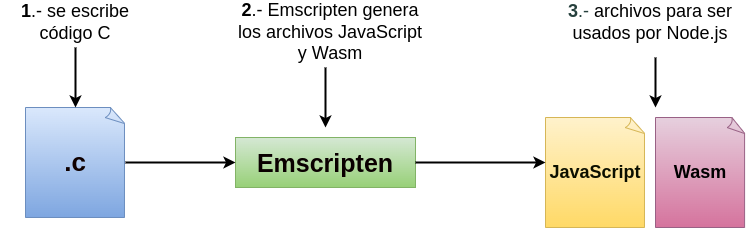
\includegraphics[scale=.47]{./Figures/Emscripten.png}
	\caption{Diagrama de funcionamiento de \textit{Emscripten}.}
	\label{fig:Emscripten}
\end{figure}


En ese sentido, para la aplicación de usuario dentro de la plataforma, cuando se ejecuta un programa de usuario, \textit{Emscripten} utiliza una función del módulo de \textit{Node.js} para la generación de un identificador único que será utilizado para los archivos generados. Este identificador esta compuesto por el prefijo \texttt{user\_} y un número entero que representa el tiempo en milisegundos. Es decir, \textit{Emscripten} creará los siguientes archivos:

\begin{itemize}

	\item Archivo \texttt{user\_tiempoenmilisegundos.js}: resultado final de la compilación y contiene el código \textit{JavaScript} que representa el programa \textit{C}.
	\item Archivo \texttt{user\_tiempoenmilisegundos.wasm}: contiene el código binario equivalente al código \textit{C} compilado. Se utiliza si el navegador del usuario admite \textit{WebAssembly} y proporciona un rendimiento mejorado en comparación con el código \textit{JavaScript} puro.
	\item Archivo \texttt{user\_tiempoenmilisegundos.js.components}: contiene datos utilizados por el programa.
	\item Archivo \texttt{user\_tiempoenmilisegundos.wasm.map}: contiene rutas de mapeos a los archivos de código \textit{C} que fueron compilados en formato \textit{Json}.
	\item Archivo \texttt{user\_tiempoenmilisegundos.wast}: representa el módulo \textit{WebAssembly} generado, pero en una representación de texto legible.
\end{itemize}

Estos archivos se ubicarán dentro del directorio de salida  \textit{outUser} que fue previamente configurado.


\subsection{JavaScript HAL}

Esta capa de programación se diseñó para proporcionar la funcionalidad de distribuir los eventos entre los componentes de la interfaz de usuario de \textit{JavaScript} y la capa \textit{C HAL}. Para lograr este objetivo se usaron las clases \textit{EventEmitter} del módulo \textit{Events} que monitorizan y activan los eventos. Además, facilita la interacción del navegador con el código \textit{JavaScript} y la actualización de la interfaz de usuario de manera flexible y eficiente.

También, la clase \textit{EventEmitter} se basa en el modelo de publicación/suscripción que se trata de un paradigma de envío de mensajes asíncrono mediante el cual un usuario publica mensajes y uno o varios objetos se suscriben a esos eventos.

En la figura \ref{fig:PublicarSuscribir} se muestra el modelo de \textit{publicación/suscripción}.

\begin{figure}[ht]
	\centering
	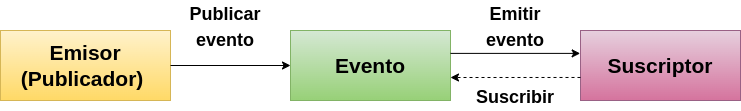
\includegraphics[scale=.49]{./Figures/PublicarSuscribir.png}
	\caption{Modelo de \textit{publicación/suscripción}.}
	\label{fig:PublicarSuscribir}
\end{figure}


Para la implementacion de esta capa de emulación, se crearon archivos \textit{JavaScript} con instancias de la clase \textit{EventEmitter}, que al utilizar el método \textit{emit} lanzan eventos con nombre. El nombre del evento es un string y permite que los oyentes registrados al evento sean notificados. La figura \ref{fig:EventemitterNodejs} muestra el diagrama de bloques de la instancia de \textit{EventEmitter} en la plataforma de emulación.

\begin{figure}[ht]
	\centering
	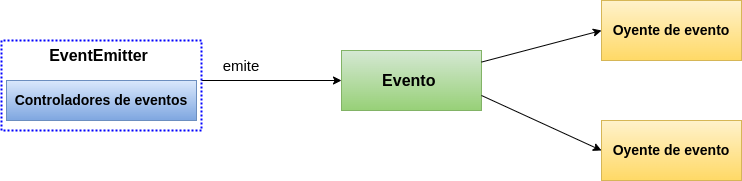
\includegraphics[scale=.49]{./Figures/EventemitterNodejs.png}
	\caption{Diagrama de bloques de \textit{EventEmitter} implementado en la plataforma.}
	\label{fig:EventemitterNodejs}
\end{figure}

En la sección de \ref{sec:caso_de_estudio}, se mostrará la implementación de este modelo en los archivos \textit{JavaScript} del emulador web.

\subsection{\textit{\textbf{sapi\_gpio}}}

Para comenzar a emular la biblioteca \textit{sapi\_gpio} del proyecto CIAA, se identificaron las funciones principales que el entorno de la plataforma web debería ofrecer al usuario. La siguiente tabla \ref{tab:sapiGPIO} muestra las funciones del archivo de código fuente \textit{sapi\_gpio} en la biblioteca \textit{\textbf{sAPI}} del proyecto CIAA que también están presentes en el emulador.


\begin{table}[h]
	\centering
	\caption[Funciones \texttt{sapi\_gpio}]{Funciones \texttt{sapi\_gpio}}
	\begin{tabular}{p{0.20\linewidth} p{0.50\linewidth}  p{0.20\linewidth}}    
		\toprule
		\textbf{Función} 	 & \textbf{Parámetros} 		& \textbf{Tipo de retorno}  \\
		\midrule
		gpioInit & gpioMap\_t pin, gpioInit\_t config 		&  bool\_t \\		
		gpioRead	 & gpioMap\_t pin			&  bool\_t \\
		gpioWrite	 & gpioMap\_t pin, bool\_t value			& bool\_t \\
		gpioToggle	 & gpioMap\_t pin				&  bool\_t \\
		\bottomrule
		\hline
	\end{tabular}
	\label{tab:sapiGPIO}
\end{table}

Además, para lograr replicar el comportamiento de cada función emulada de manera que, al invocarlas, produzcan resultados similares a los que se obtendrían al utilizar las funciones con el hardware físico, se utilizó la capa de \textit{C HAL}. Esta capa interactúa con la capa \textit{Javascript HAL}, que se encarga de comunicarse con la interfaz de usuario, permitiendo mostrar el comportamiento de los pines GPIO programados en la aplicación del usuario.

Entonces, se utilizó la capa de emulación correspondiente a \textit{C HAL} para emular las siguientes funcionalidades:

\begin{itemize}
	\item \texttt{Chip\_GPIO\_Init(LPC\_GPIO\_PORT)}se utiliza para inicializar y configurar el hardware de los pines GPIO de la placa. En la capa de emulación \textit{C HAL}, utilizando  \textit{Emscripten}, también se realizaron configuraciones de variables para representar los tipos de pines e inicializarlos.
	
	\item \texttt{Chip\_GPIO\_SetDir (LPC\_GPIO\_PORT, gpioPort, \newline (1 \<<\<<  gpioPin), GPIO\_OUTPUT)}se utiliza para establecer si un pin GPIO se utilizará para recibir datos (entrada) o enviar datos (salida). De manera similar, en la capa de abstracción de datos en \textit{C}, se implementaron configuraciones similares para la capa \textit{Javascript HAL} usando las macros de \textit{Emscripten}.
	
	\item \texttt{Chip\_GPIO\_SetPinState(LPC\_GPIO\_PORT, gpioPort, \newline gpioPin, 0)} se utiliza para gestionar el estado de los pines GPIO, permitiendo configurarlos como salidas y establecer su valor (alto o bajo). En la capa de abstracción de datos \textit{C}, esta función actualiza la estructura de datos utilizada para almacenar información sobre la configuración de los pines GPIO. Además, registra el valor del pin especificado como parámetro.

	\item \texttt{Chip\_GPIO\_ReadPortBit(LPC\_GPIO\_PORT, gpioPort, \newline gpioPin)} se utiliza para obtener el estado actual de un pin GPIO específico en la placa, lo que permite leer datos provenientes de dispositivos externos o de otros componentes conectados a los pines GPIO. En la capa de emulación \textit{C HAL}, se emula la lectura del estado de un pin GPIO utilizando la información almacenada en la estructura de datos.
\end{itemize}


Para emular las funciones mencionadas anteriormente, se utilizó la macro \newline \texttt{EM\_ASM\_}, mediante la cual se incrustó código \textit{JavaScript} directamente en el código \textit{C}. Este código \textit{JavaScript} incrustado se compila junto con el código C y se ejecutará en el entorno de ejecución de \textit{Emscripten}  cuando la aplicación de usuario invoque a esas funciones. La figura \ref{fig:gpioEmscripten} muestra el diagrama de bloques de la macro \texttt{EM\_ASM\_}.

\hfill \break


\begin{figure}[ht]
	\centering
	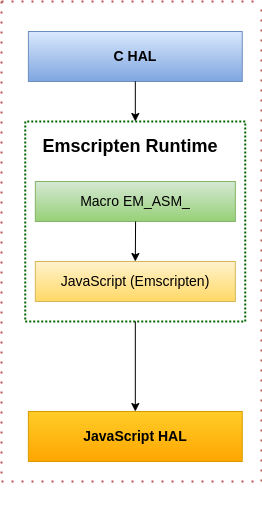
\includegraphics[scale=.40]{./Figures/gpioEmscripten.png}
	\caption{Diagrama de bloques de la macro \texttt{EM\_ASM\_}.}
	\label{fig:gpioEmscripten}
\end{figure}


Asimismo, para emular las interacciones entre la interfaz de usuario y las GPIO TEC1, TEC2, TEC3 y TEC4, se utilizó en la capa \textit{C HAL} la macro \newline \texttt{EMSCRIPTEN\_KEEPALIVE}. Su funcionamiento se explica en la siguiente sección \ref{sec:sapi_tick}. 

A continuación, en la capa \textit{Javascript HAL}, se distribuyen eventos a la capa \textit{Javascript UI} para notificarle que el pin GPIO ha sido configurado desde la capa \textit{C HAL}. Estos eventos incluyen información que será útil para gestionar los pines GPIO en la capa de interfaz de usuario. La figura \ref{fig:gpioEmit} muestra el diagrama de bloques del envío de eventos de la capa \textit{Javascript HAL} a la capa \textit{Javascript UI}.

\begin{figure}[ht]
	\centering
	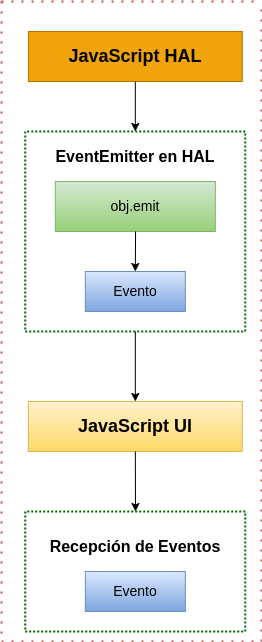
\includegraphics[scale=.40]{./Figures/gpioEmit.png}
	\caption{Diagrama de bloques del envío de eventos de la capa \textit{Javascript HAL}.}
	\label{fig:gpioEmit}
\end{figure}

Por consiguiente, en la capa \textit{Javascript UI} se manipulan esos eventos, y en consecuencia, se actualiza la interfaz de la plataforma web para mostrar al usuario los cambios.

\subsection{\textit{\textbf{sapi\_tick}}}
\label{sec:sapi_tick}

En la tabla \ref{tab:sapiTick} se puede observar las funciones del archivo de código fuente \texttt{sapi\_tick} en la biblioteca \textit{\textbf{sAPI}} del proyecto CIAA y en el emulador.

\begin{table}[h]
	\centering
	\caption[Funciones \texttt{sapi\_tick}]{Funciones \texttt{sapi\_tick}}
	\begin{tabular}{p{0.20\linewidth} p{0.50\linewidth}  p{0.20\linewidth}}    
		\toprule
		\textbf{Función} 	 & \textbf{Parámetros} 		& \textbf{Tipo de retorno}  \\
		\midrule
		tickInit & tick\_t tickRateMSvalue 		&  bool\_t \\		
		tickRead	 & void				&  tick\_t \\
		tickWrite	 & tick\_t ticks 				& void \\
		tickCallbackSet	 & callBackFuncPtr\_t tickCallback, void* tickCallbackParams				&  bool\_t \\
		tickPowerSet & bool\_t power 		&  void \\	
		\bottomrule
		\hline
	\end{tabular}
	\label{tab:sapiTick}
\end{table}

Para emular a nivel de API, se tuvo como objetivo replicar el comportamiento de la función \texttt{tickInit}, la cual se encarga de la inicialización y configuración de la interrupción del temporizador \texttt{SysTick\_Config} en la placa física. Sin embargo, al realizar la emulación en la plataforma web, esta función no se encuentra disponible de forma nativa. Por lo tanto, fue necesario emular su comportamiento y proporcionar una alternativa compatible.

Para emular la funcionalidad de \texttt{SysTick\_Config}, se utilizó la capa de emulación correspondiente a \textit{C HAL}. Esta capa de emulación permitió ejecutar código \textit{JavaScript} en el contexto de \textit{Emscripten}, lo que posibilitó replicar el comportamiento del temporizador \textit{SysTick}. 

Una vez habilitada la interrupción del temporizador, se realiza una invocación periódica a la función \texttt{tickerCallback}, que tiene la misma implementación que en \texttt{sapi\_tick} de la biblioteca \textit{\textbf{sAPI}} del proyecto CIAA. La función \newline \texttt{tickerCallback} realiza las siguientes acciones: incrementa los contadores de ticks y, si el puntero \texttt{tickHookFunction} no es nulo, ejecuta la función establecida como \textit{calback} mediante la función de \textit{\textbf{sAPI}} \texttt{tickCallbackSet()}, pasando los parámetros \texttt{callBackFuncParams}. En consecuencia, esto permite la ejecución de tareas específicas programadas por el usuario en cada interrupción del temporizador periódico.

En el capítulo 4 se detallarán las diferencias encontradas al realizar las pruebas entre la placa y el emulador utilizando estas funciones.

En el contexto de la emulación a nivel de API, para implementar las demás bibliotecas de las \textit{\textbf{sAPI}}, se siguió el mismo esquema utilizado en \texttt{sapi\_tick}. Primeramente, se identificaron las funciones que requerían interacción con el hardware de la placa. Luego, en la capa \textit{C HAL} se implementaron funciones de emulación con \textit{Emscripten} para reflejar el comportamiento del hardware.

Para emular el comportamiento de la interrupción del temporizador \textit{SysTick} y proporcionar la invocación periódica a la función \texttt{tickerCallback} de \textit{sapi\_tick}, se utilizó la macro \texttt{EMSCRIPTEN\_KEEPALIVE} de \textit{Emscripten}, que le dice al compilador de \textit{Emscripten} que conserve la función marcada con esta macro en el código compilado, incluso si no es accedida desde el código \textit{JavaScript} del lado del cliente.

Es decir, cuando la función marcada con la macro \texttt{EMSCRIPTEN\_KEEPALIVE} sea invocada desde la capa \textit{JavaScript HAL}, llamará a la función \texttt{tickerCallback} de la biblioteca \textit{C} y la ejecutará. En la figura \ref{fig:tickerCallback} se muestra el funcionamiento de \texttt{EMSCRIPTEN\_KEEPALIVE}. 


\begin{figure}[ht]
	\centering
	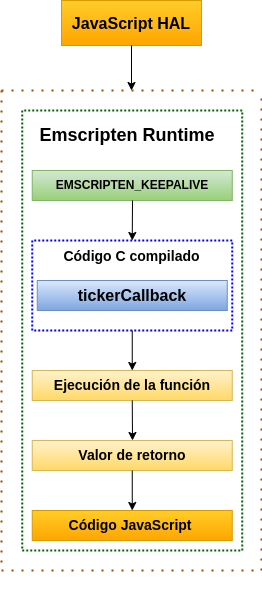
\includegraphics[scale=.55]{./Figures/tickerCallback.png}
	\caption{Diagrama de bloques \texttt{EMSCRIPTEN\_KEEPALIVE}.}
	\label{fig:tickerCallback}
\end{figure}



Para lograr la interacción con la capa de emulación \textit{C HAL}, y realizar la invocación periódica a la función que usa la macro \texttt{EMSCRIPTEN\_KEEPALIVE} de \textit{Emscripten} se configuró en esta capa de desarrollo un temporizador de \textit{JavaScript}.

Además, dentro del temporizador, se utilizó la función \texttt{ccall} de \textit{Emscripten}, que permite invocar a la funcion \texttt{tickerCallback} desde el código \textit{C} compilado con \textit{Emscripten}. 

A continuacion, se muestra en la figura  \ref{fig:ccall} el funcionamiento de \texttt{ccall}. 

\hfill \break
\hfill \break
\hfill \break
\hfill \break

\begin{figure}[ht]
	\centering
	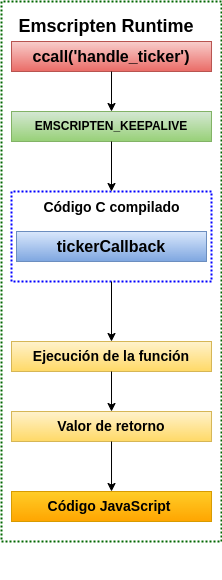
\includegraphics[scale=.49]{./Figures/ccall.png}
	\caption{Diagrama de bloques de la función \textit{ccall}.}
	\label{fig:ccall}
\end{figure}

Sin embargo, debido a la naturaleza asíncrona de \textit{JavaScript} y al uso de la función \texttt{ccall}, la función no mantiene el contexto entre las ejecuciones del temporizador. En consecuencia, cada vez que se reinicia el temporizador y se ejecuta la función  \texttt{tickerCallback}, la tarea específica programada por el usuario comienza desde el principio en lugar de continuar desde el punto donde quedó anteriormente. 

\subsection{\textit{\textbf{sapi\_delay}}}

La tabla \ref{tab:sapiDelay} expone las funciones del archivo de código fuente \texttt{sapi\_delay} en la biblioteca \textit{\textbf{sAPI}} del proyecto CIAA y en el emulador.

\begin{table}[h]
	\centering
	\caption[Funciones \texttt{sapi\_delay}]{Funciones \texttt{sapi\_delay}}
	\begin{tabular}{p{0.30\linewidth} p{0.40\linewidth}  p{0.20\linewidth}}    
		\toprule
		\textbf{Función} 	 & \textbf{Parámetros} 		& \textbf{Tipo de retorno}  \\
		\midrule
		delayInaccurateMs & tick\_t delay\_ms 		&  void \\		
		delayInaccurateUs	 & tick\_t delay\_us			&  void \\
		delayInaccurateNs	 & tick\_t delay\_ns				& void \\
		delay	 & tick\_t duration\_ms				&  void \\
		delayInit & delay\_t * delay, tick\_t duration 		&  void \\
		delayRead & delay\_t * delay 		&  bool\_t \\
		delayWrite & delay\_t * delay, tick\_t duration 		&  void \\	
		\bottomrule
		\hline
	\end{tabular}
	\label{tab:sapiDelay}
\end{table}

La función \texttt{delay} en la biblioteca \textit{\textbf{sAPI}} del proyecto CIAA crea una pausa en la ejecución del programa durante el tiempo especificado en \texttt{duration\_ms} implementando un bucle de espera. Este bucle se ejecutará mientras la diferencia de tiempo entre \texttt{tickRead()} y startTime(inicio actual de \texttt{tickRead()} sea menor que \texttt{duration\_ms/ tickRateMS}.

Sin embargo, cuando \textit{Emscripten} compila código \textit{C} a \textit{JavaScript}, la función \texttt{delay} tal como está escrita, causa que la ejecución de la plataforma web se bloquee o congele. Esto se debe a que la función \texttt{tickRead()} no se actualiza a la velocidad que se espera, lo que lleva a que se obtenga el mismo valor repetidamente. Es decir, debido a la naturaleza asincrónica de \textit{JavaScript} y al no tener una pausa controlada en el bucle (como \texttt{delay(1)}), \textit{JavaScript} no tiene tiempo suficiente para actualizar el valor de \texttt{tickRead()} entre iteraciones. De esta manera,  el bucle \texttt{while} se queda esperando activamente e impide al navegador atender otros eventos.

Por esta razón, se decidio usar en las funciones de espera,  las funciones nativas de \textit{Emscripten} usando la capa de emulación \textit{C HAL}, que se ira detallando en la siguiente sección. En consecuencia, se aprovecho su eficiencia y precisión.

Para emular las funciones de espera de la biblioteca \textit{C} se implemento la función \texttt{emscripten\_sleep}, que utiliza funciones asincrónicas internas de \textit{Emscripten} para realizar pausas. 

Por lo tanto, permite al navegador atender otros eventos mientras el programa se encuentra en espera. Es decir, evita el bloqueo de la ejecución del resto del código y también, que la página no responda.

Además, proporciona pausas precisas, debido a que, \textit{Emscripten}  utiliza las capacidades de temporización del navegador para garantizar que el tiempo indicado sea realizado.

La figura \ref{fig:emscriptenDelay} representa el funcionamiento de  \texttt{emscripten\_sleep}. 


\begin{figure}[ht]
	\centering
	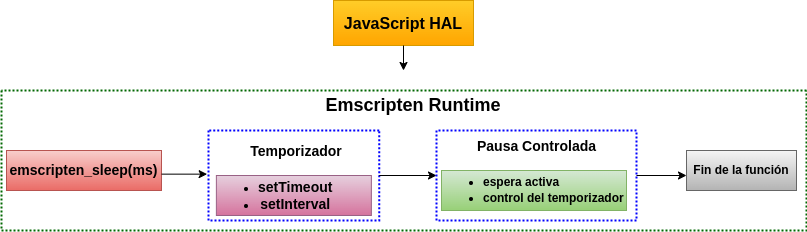
\includegraphics[scale=.50]{./Figures/emscriptenDelay.png}
	\caption{Diagrama de bloques \texttt{emscripten\_sleep.}}
	\label{fig:emscriptenDelay}
\end{figure}




\subsection{\textit{\textbf{freertos}}}

Para emular la funcionalidad de las tareas de \textit{freeRTOS} en el contexto del emulador web, se utilizó la biblioteca de eventos de \textit{mbed}. Entonces, para las funciones \texttt{xTaskCreate} y \texttt{xTaskCreateStatic}, se programaron funciones periódicas utilizando las siguientes funciones de la biblioteca de \textit{Mbed events}: 

 
 \begin{itemize}
	\item \texttt{int equeue\_create}:  crea una cola de eventos, configura e inicializa los recursos de plataforma necesarios, como semáforos y mutexes.
	
	\item \texttt{int equeue\_call\_every}:  se utiliza para crear un evento periódico en la cola de eventos equeue, programando llamadas repetidas a una función en intervalos regulares.
	
	\item \texttt{int equeue\_post}: permite publicar un evento en la cola de eventos equeue, estableciendo el tiempo y estableciendo el evento en la cola para su posterior procesamiento.
	
	\item \texttt{void equeue\_dispatch}: se encarga de despachar los eventos en la cola de eventos equeue de manera continua, verificando los tiempo y realizando acciones específicas según la configuración.

	\item \texttt{void equeue\_destroy}: permite liberar y limpiar todos los recursos asociados a una cola de eventos, libera los mutexes, semáforos y memoria asignada.
\end{itemize}

Estas funciones permiten ejecutar tareas periódicas en intervalos de tiempo regulares, lo que proporcionó una aproximación simplificada a la funcionalidad de tareas en el emulador web. Aunque esta solución no ofrece todas las características de un sistema operativo de tiempo real completo como \textit{freeRTOS}, fue adecuada para emular el funcionamiento de programas de usuario simples.

Es importante destacar que la implementación de tareas en el emulador web tiene una limitación significativa. Debido a que solo puede ejecutar un subproceso (hilo de ejecución) a la vez, no es posible que se ejecuten tareas simultáneas. Esto significa que, a diferencia del sistema operativo de tiempo real \textit{freeRTOS}, donde se pueden crear múltiples tareas que se ejecutan de manera concurrente, en el emulador web solo es posible ejecutar una sola tarea. Por lo tanto, esta solución es adecuada para programas de usuario simples que no requieran multitarea.


La tabla \ref{tab:ConceptosRTOS} expone algunos de los conceptos importantes de \textit{freeRTOS} que se cumplen en el emulador.

\begin{table}[h]
\centering
\caption[Conceptos importantes de \textit{freeRTOS} que se cumplen en el emulador.]{Conceptos importantes de \textit{freeRTOS} que se cumplen en el emulador.}
\begin{tabular}{p{0.45\linewidth} p{0.15\linewidth}  p{0.15\linewidth}}
\toprule
\textbf{Capacidades} 
& \textbf{\textit{freeRTOS}}
& \textbf{Emulador}
\\
\midrule
Multitareas & Si & No  \\
Funciones de espera &  Si & Si \\
Cambio de contexto &  Si & Si \\
Tarea de procesamiento continuo &  Si & Si \\
Manejo de prioridades & Si & No  \\
\bottomrule
\hline
\end{tabular}
\label{tab:ConceptosRTOS}
\end{table}

En el emulador, se encuentran implementados varios conceptos importantes de \textit{freeRTOS}, como funciones de espera y cambio de contexto. Sin embargo, en esta primera versión del emulador, no se han incluido el manejo de multitareas y de prioridades presentes en \textit{freeRTOS}.


\subsection{\textit{\textbf{sapi\_dht11}}}

Al emular los periféricos externos de la biblioteca \textit{\textbf{sAPI}} del proyecto CIAA, se continuó con la misma lógica de programación utilizada para interactuar con los periféricos de la placa EDU-CIAA-NXP. Asimismo, se mapearon las funcionalidades ofrecidas por la biblioteca \textit{\textbf{sAPI}} a la plataforma web. En la siguiente tabla \ref{tab:sapiDht11} se muestran las funciones presentes en ambas plataformas.


\begin{table}[h]
	\centering
	\caption[Funciones \texttt{sapi\_dht11}]{Funciones \texttt{sapi\_dht11}}
	\begin{tabular}{p{0.20\linewidth} p{0.50\linewidth}  p{0.20\linewidth}}    
		\toprule
		\textbf{Función} 	 & \textbf{Parámetros} 		& \textbf{Tipo de retorno}  \\
		\midrule
		dht11Init & int32\_t gpio		&  void \\		
		dht11Read	 & float *phum, float *ptemp	&  bool\_t \\
		\bottomrule
		\hline
	\end{tabular}
	\label{tab:sapiDht11}
\end{table}

En esta primera versión de la plataforma web, no se ofrece la capacidad gráfica de las interacciones virtuales entre la placa y los periféricos externos. Sin embargo, el usuario debe realizar las configuraciones manualmente, eligiendo las conexiones correctas, que luego serán verificadas en la capa de \textit{JavaScript UI}.
Además, en \textit{JavaScript UI}, principalmente se centró el trabajo de emular el envío de los datos de temperatura y humedad del sensor DHT11 al microcontrolador.


Entonces, en la capa de abstracción de datos \textit{C HAL} se implementó la lectura de los datos provenientes de la capa \textit{JavaScript HAL} al usar la macro \texttt{EM\_ASM\_INT} de \textit{Emscripten}. A continuación, en la figura \ref{fig:dht11Emscripten} se presenta el diagrama de bloques de la macro \texttt{EM\_ASM\_INT}.

\begin{figure}[ht]
	\centering
	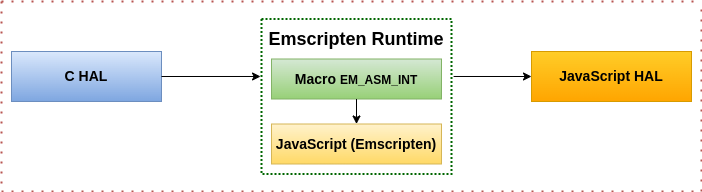
\includegraphics[scale=.53]{./Figures/dht11Emscripten.png}
	\caption{Diagrama de bloques de la macro \texttt{EM\_ASM\_INT}.}
	\label{fig:dht11Emscripten}
\end{figure}

La capa \textit{JavaScript HAL} recibe los datos enviados desde \textit{JavaScript UI} y los transmite a la capa \textit{C HAL}. La generación de los datos  emulados de temperatura y humedad, se realiza en \textit{JavaScript UI} a través de dos opciones elegidas por el usuario:
 
 \begin{itemize}
	\item Obtener los datos de temperatura y humedad local conectándose a una central meteorológica a través de la geolocalización del navegador del usuario. Sin embargo, si el servidor donde se encuentra desplegada la plataforma web no puede acceder al servicio de geolocalización del navegador o el usuario no permite el acceso, entonces se realizará la consulta a la central meteorológica utilizando la ubicación predeterminada de la ciudad de Buenos Aires.
	
	\item Generar los datos manualmente haciendo click en la interfaz gráfica que representa a la temperatura y humedad. De esta manera, el usuario puede generar los datos según su elección.
\end{itemize}

En la figura \ref{fig:uiDht11} se muestra el diagrama de bloques de la capa de interfaz de usuario \textit{JavaScript UI} con las dos opciones de usuario.

\begin{figure}[ht]
	\centering
	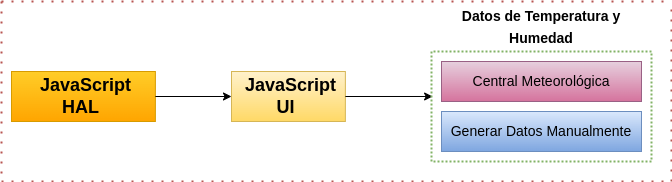
\includegraphics[scale=.57]{./Figures/uiDht11.png}
	\caption{Diagrama de bloques de la capa \textit{JavaScript UI} con las dos opciones para el usuario.}
	\label{fig:uiDht11}
\end{figure}

\subsection{\textit{\textbf{sapi\_adc}}}

Para comenzar, se realizó el mapeo de las funciones del módulo de la biblioteca \textit{\textbf{sAPI}} a la plataforma web. La tabla \ref{tab:sapiADC} expone las funciones presentes en ambas plataformas.


\begin{table}[h]
	\centering
	\caption[Funciones \texttt{sapi\_adc}]{Funciones \texttt{sapi\_adc}}
	\begin{tabular}{p{0.20\linewidth} p{0.50\linewidth}  p{0.20\linewidth}}    
		\toprule
		\textbf{Función} 	 & \textbf{Parámetros} 		& \textbf{Tipo de retorno}  \\
		\midrule
		adcInit & adcInit\_t config		&  void \\		
		adcRead	 & adcMap\_t analogInput	&  uint16\_t \\
		\bottomrule
		\hline
	\end{tabular}
	\label{tab:sapiADC}
\end{table}

El módulo \textit{adc} fue implementado en el emulador  para ser utilizado con varios periféricos dentro del entorno web, incluyendo el potenciómetro, el termistor NTC y el joystick. De esta manera, permite al usuario realizar pruebas de funcionamiento de un \textit{adc} real. 

Luego, se implementaron las funciones de inicialización y de lectura del componente \textit{adc}  en la capa \textit{C HAL}. Posteriormente, son utilizadas por la capa \textit{JavaScript HAL} para la interacción con el hardware y permitir al usuario trabajar con los periféricos externos en un entorno web. La figura \ref{fig:adcEmscripten} presenta el diagrama de bloques de las capas: \textit{C HAL} y \textit{JavaScript HAL} para el \textit{adc}.

\begin{figure}[ht]
	\centering
	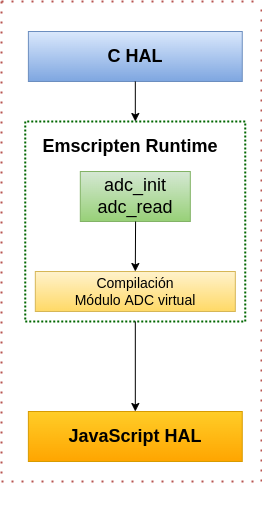
\includegraphics[scale=.53]{./Figures/adcEmscripten.png}
	\caption{Diagrama de bloques de \textit{C HAL} y \textit{JavaScript HAL} para el módulo \textit{adc}.}
	\label{fig:adcEmscripten}
\end{figure}

En la capa \textit{JavaScript UI}, se implementó la obtención de datos para los periféricos externos que interactúan con el \textit{adc}. Por ejemplo, para el potenciómetro, los datos son establecidos por el usuario a través de la interfaz gráfica utilizando el componente HTML  \textit{input} de tipo \textit{range}. De esta manera, el usuario al deslizar este componente dentro de un rango mínimo y máximo establecido, se va realizando el siguiente cálculo para obtener el valor del \textit{adc} correspondiente:

\begin{lstlisting}[caption={Cálculo del ADC para el potenciómetro.}]
  window.JSHal.gpio.write(self.dataPin.ADC, range.value/ 3.3 * 1023);
\end{lstlisting}

En consecuencia, los cálculos actualizados se muestran en la interfaz gráfica del emulador web.

En el caso del termistor NTC, se implementó en la interfaz grafica un elemento gráfico (termómetro) para representar la temperatura en grados celsius. A medida que el usuario ajusta el termómetro, la temperatura en kelvin se va actualizando en función de la temperatura en grados celsius y, además, el valor del \textit{adc} se actualiza mediante la siguiente función:

\begin{lstlisting}[caption={Cálculo ADC del termistor NTC.}]
     ThermistorNTC.prototype.updateSampleADC= function(R_NTC) {
        let R_NTC_float = parseFloat(R_NTC);
        let R_10k_float = parseFloat(R_10k);
        let Vsupply_float = parseFloat(Vsupply);    
        let VoutT = (R_NTC_float * Vsupply_float) / (R_10k_float + R_NTC_float);
        Vout = parseFloat(VoutT.toFixed(2)); 

        this.sample = parseFloat((Vout * 1023.0 / Vsupply).toPrecision(4));
        console.log('this.sample ', this.sample);
        window.JSHal.gpio.write(this.dataPin.ADC, this.sample);     
    };
\end{lstlisting}

Además, se implementó un componente web para el joystick, encargado de gestionar los movimientos y acciones en las interacciones con el usuario. Los datos de los movimientos de los ejes X e Y del joystick son obtenidos y se utilizan para realizar cálculos de voltajes en las respectivas resistencias de cada eje, así como también, para calcular el valor del \textit{adc}. A modo de referencia se muestra las cálculos que se hicieron para el eje X del joystick:

\begin{lstlisting}[caption={Cálculo de la resistencia del eje X y del ADC.}]
            var VRx = Joy.GetVRx();
            var voltage = (Math.floor(VRx/ 3.3 * 1023)* 3.3 / 1023.0).toFixed(2);
            joyVRx.textContent = voltage;
            joyADCx.textContent = Math.trunc(VRx/ 3.3 * 1023);
            window.JSHal.gpio.write(self.dataPin.ADCx, VRx/ 3.3 * 1023);
\end{lstlisting}

Luego, para cada periférico externo, el cálculo del \textit{adc} es envíado a la capa \textit{JavaScript HAL}.
En la figura \ref{fig:uiADC} se muestra el diagrama de bloques con la interaccion de ambas capas de desarrollo.

\begin{figure}[ht]
	\centering
	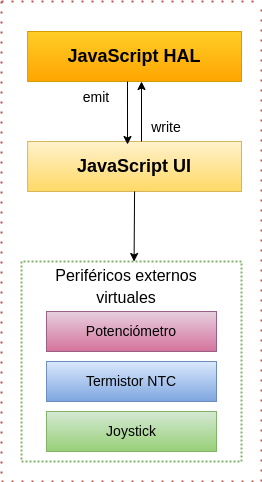
\includegraphics[scale=.57]{./Figures/uiADC.png}
	\caption{Diagrama de bloques con la interaccion de las capas  \textit{JavaScript HAL} y \textit{JavaScript UI}.}
	\label{fig:uiADC}
\end{figure}

\hfill \break
\hfill \break
\hfill \break
\hfill \break
\hfill \break
\hfill \break
\hfill \break
\hfill \break
\hfill \break
\hfill \break
\hfill \break
\hfill \break

\subsection{Tabla de Periféricos}

La siguiente tabla \ref{tab:perifericosInternosMBED} expone los  periféricos internos implementados actualmente en \textit{Mbed Simulator}.

\begin{table}[h]
\centering
\caption[Comparación de características de periféricos internos implementados en \textit{Mbed Simulator}]{Comparación de características de Periféricos internos implementados en \textit{Mbed Simulator}}
\begin{tabular}{p{0.24\linewidth} p{0.14\linewidth}  p{0.14\linewidth}  p{0.14\linewidth}}
\toprule
\textbf{Periféricos} 
& \textbf{Velocidad y tiempo real}
& \textbf{Responde a eventos}
\\
\midrule
GPIO & Si & Si  \\
UART & Si & Si \\
BUTTON & SI & Si \\
ADC & Si & Si \\
DAC & Si & Si \\
PWM & Si & Si \\ 
\bottomrule
\hline
\end{tabular}
\label{tab:perifericosInternosMBED}
\end{table}


En la figura \ref{fig:GPIOMbed} se muestra el funcionamiento de GPIO y en la figura \ref{fig:PMWMbed} expone el funcionamiento de PWM del \textit{Mbed Simulator}.

\hfill \break
\hfill \break
\hfill \break
\hfill \break
\hfill \break

\begin{figure}[ht]
	\centering
	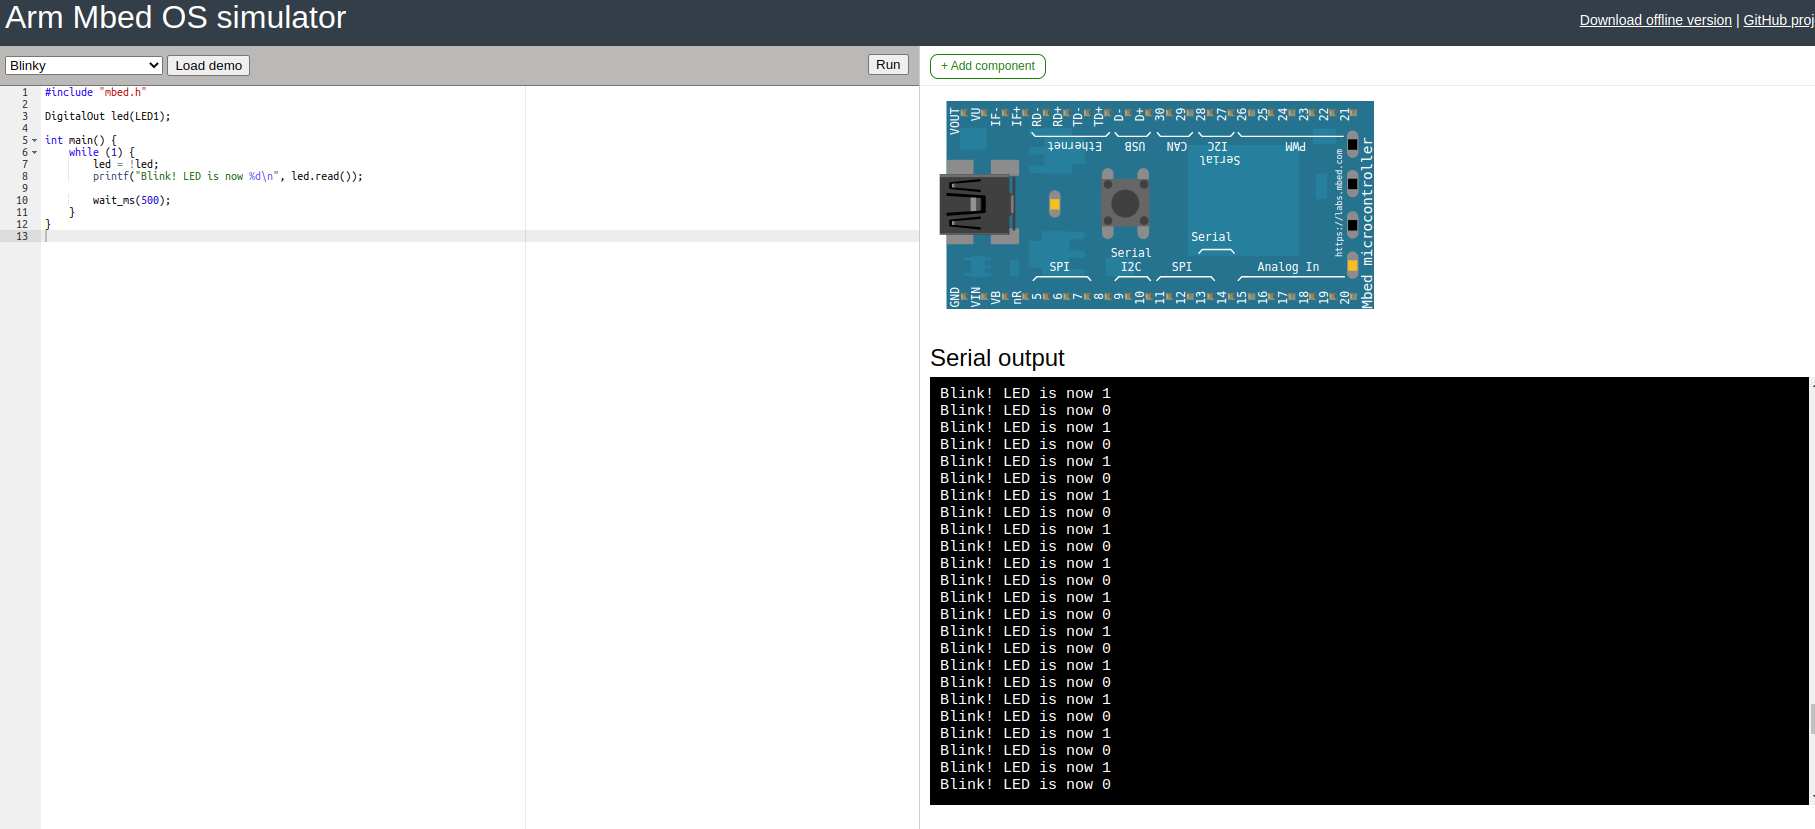
\includegraphics[scale=.24]{./Figures/GPIOMbed.png}
	\caption{Funcionamiento GPIO en \textit{Mbed Simulator}.}
	\label{fig:GPIOMbed}
\end{figure}

\begin{figure}[ht]
	\centering
	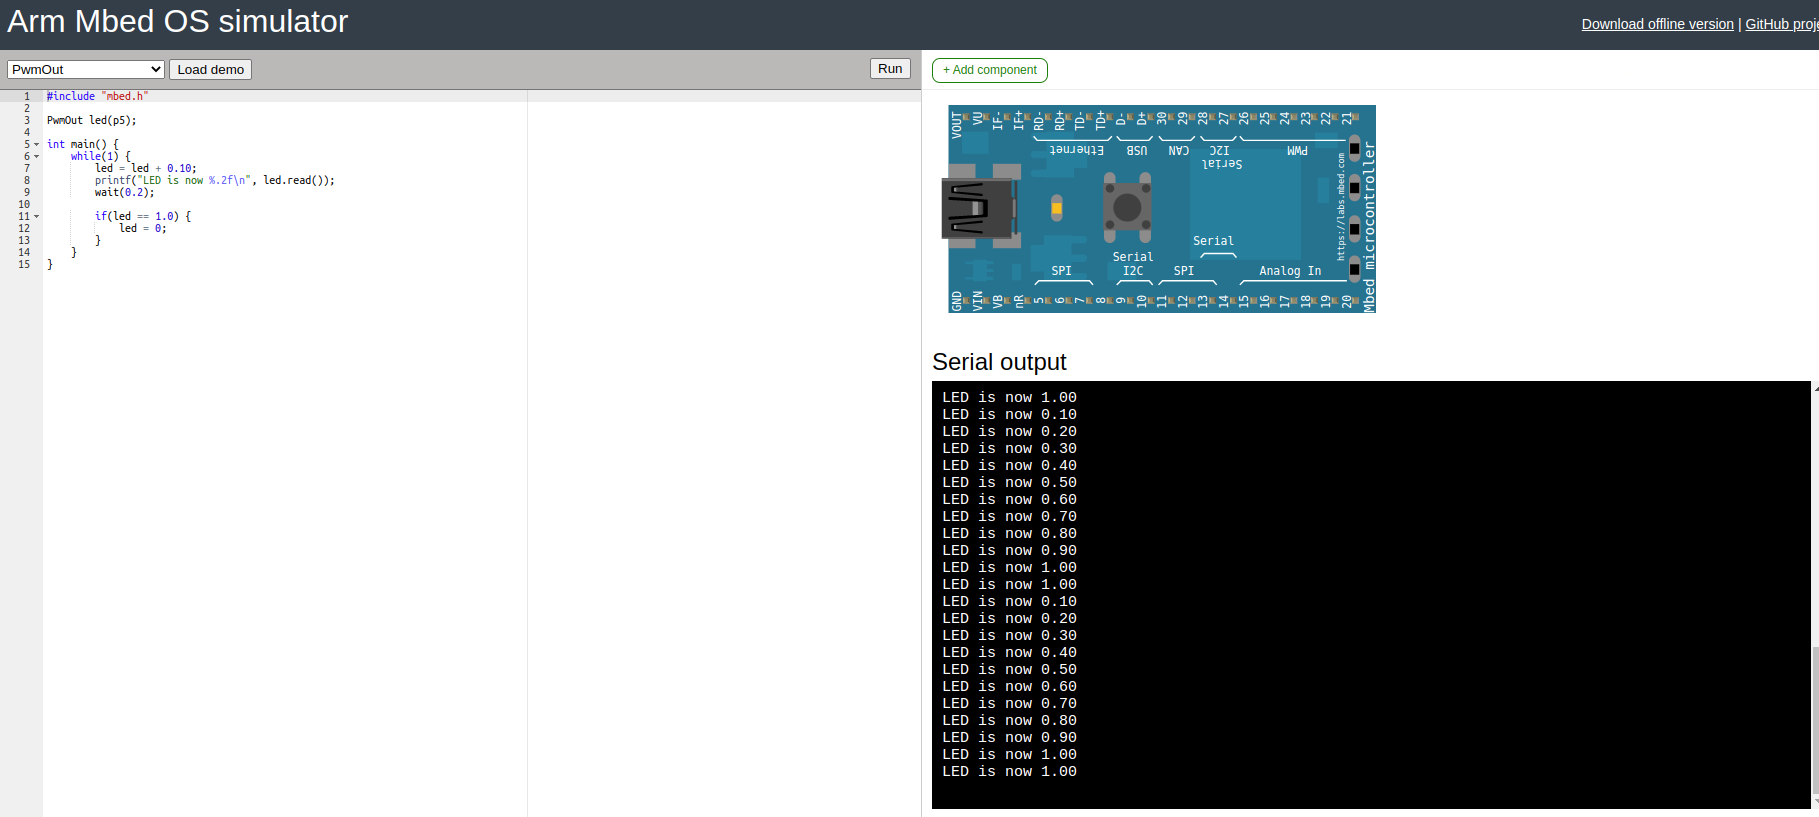
\includegraphics[scale=.24]{./Figures/PMWMbed.png}
	\caption{Funcionamiento PWM en \textit{Mbed Simulator}.}
	\label{fig:PMWMbed}
\end{figure}





Además, en la tabla \ref{tab:perifericosExternosMBED} expone los  periféricos externos implementados actualmente en \textit{Mbed Simulator}.


\begin{table}[h]
\centering
\caption[Comparación de características de Periféricos externos implementados en \textit{Mbed Simulator}]{Comparación de características de Periféricos externos implementados en \textit{Mbed Simulator}}
\begin{tabular}{p{0.30\linewidth} p{0.14\linewidth}  p{0.14\linewidth}  p{0.14\linewidth}}
\toprule
\textbf{Periféricos} 
& \textbf{Velocidad y tiempo real}
& \textbf{Responde a eventos}
\\
\midrule
DHT11 & Si & Si  \\
LCD Display C12832 & Si & Si  \\
LED & No & Si \\
Thermistor & Si & Si \\
SHT31 & Si & Si \\
Touch Screen ST7789H2 & Si & Si \\
\bottomrule
\hline
\end{tabular}
\label{tab:perifericosExternosMBED}
\end{table}

La figura \ref{fig:perifericosMbed} muestra los periféricos externos de \textit{Mbed Simulator}.
\hfill \break
\hfill \break
\hfill \break
\hfill \break
\hfill \break

\begin{figure}[ht]
	\centering
	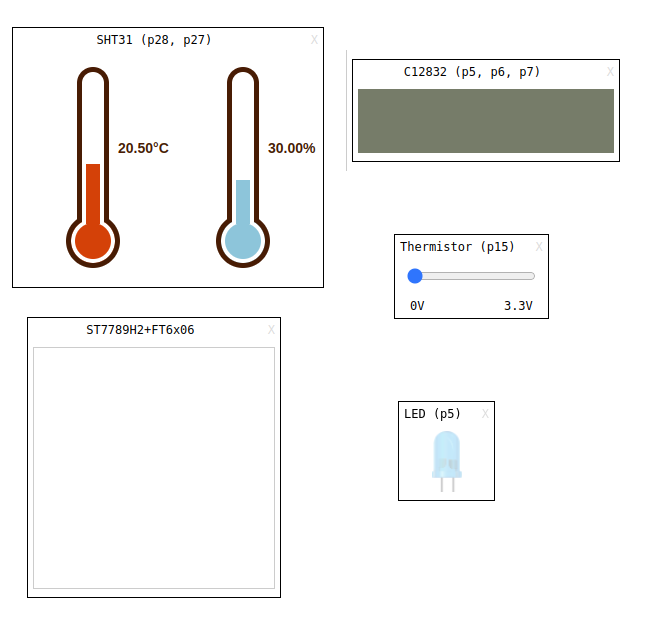
\includegraphics[scale=.70]{./Figures/perifericosMBED.png}
	\caption{Periféricos externos de \textit{Mbed Simulator}.}
	\label{fig:perifericosMbed}
\end{figure}

En la siguiente tabla \ref{tab:perifericosInternosCIAA} se exponen los  periféricos internos implementados en la primera versión de la plataforma de emulación web de la placa EDU-CIAA.

\begin{table}[h]
\centering
\caption[Comparación de características de periféricos internos del Emulador EDU-CIAA]{Comparación de características de Periféricos}
\begin{tabular}{p{0.24\linewidth} p{0.14\linewidth}  p{0.14\linewidth}  p{0.14\linewidth}}
\toprule
\textbf{Periféricos} 
& \textbf{Velocidad y tiempo real}
& \textbf{Responde a eventos}
\\
\midrule
GPIO & Si & Si  \\
UART & Si & Si \\
BUTTON & SI & Si \\
RTC & Si & Si  \\
SYSTICK & No & Si \\
ADC & Si & Si \\
DAC & Si & Si \\
\bottomrule
\hline
\end{tabular}
\label{tab:perifericosInternosCIAA}
\end{table}


Además, la siguiente tabla \ref{tab:perifericosExternosCIAA} se exponen los  periféricos externos implementados en la primera versión de la plataforma de emulación web.

\hfill \break
\hfill \break
\hfill \break
\hfill \break

\begin{table}[h]
\centering
\caption[Comparación de características de periféricos externos del Emulador EDU-CIAA]{Comparación de características de Periféricos externos del Emulador EDU-CIAA}
\begin{tabular}{p{0.30\linewidth} p{0.14\linewidth}  p{0.14\linewidth}  p{0.14\linewidth}}
\toprule
\textbf{Periféricos} 
& \textbf{Velocidad y tiempo real}
& \textbf{Responde a eventos}
\\
\midrule
DHT11 & Si & Si  \\
LCD & Si & Si  \\
LED & Si & Si  \\
SYSTICK & No & Si \\
LCD DISPLAY 128x64 & Si & Si \\
LCD DISPLAY 20x4 & Si & Si \\
Thermistor NTC & Si & Si \\
Potentiometer & Si & Si \\
Joystick & Si & Si \\
\bottomrule
\hline
\end{tabular}
\label{tab:perifericosExternosCIAA}
\end{table}


La figura \ref{fig:perifericosCIAA} muestra los periféricos externos del emulador web EDU-CIAA.

\begin{figure}[ht]
	\centering
	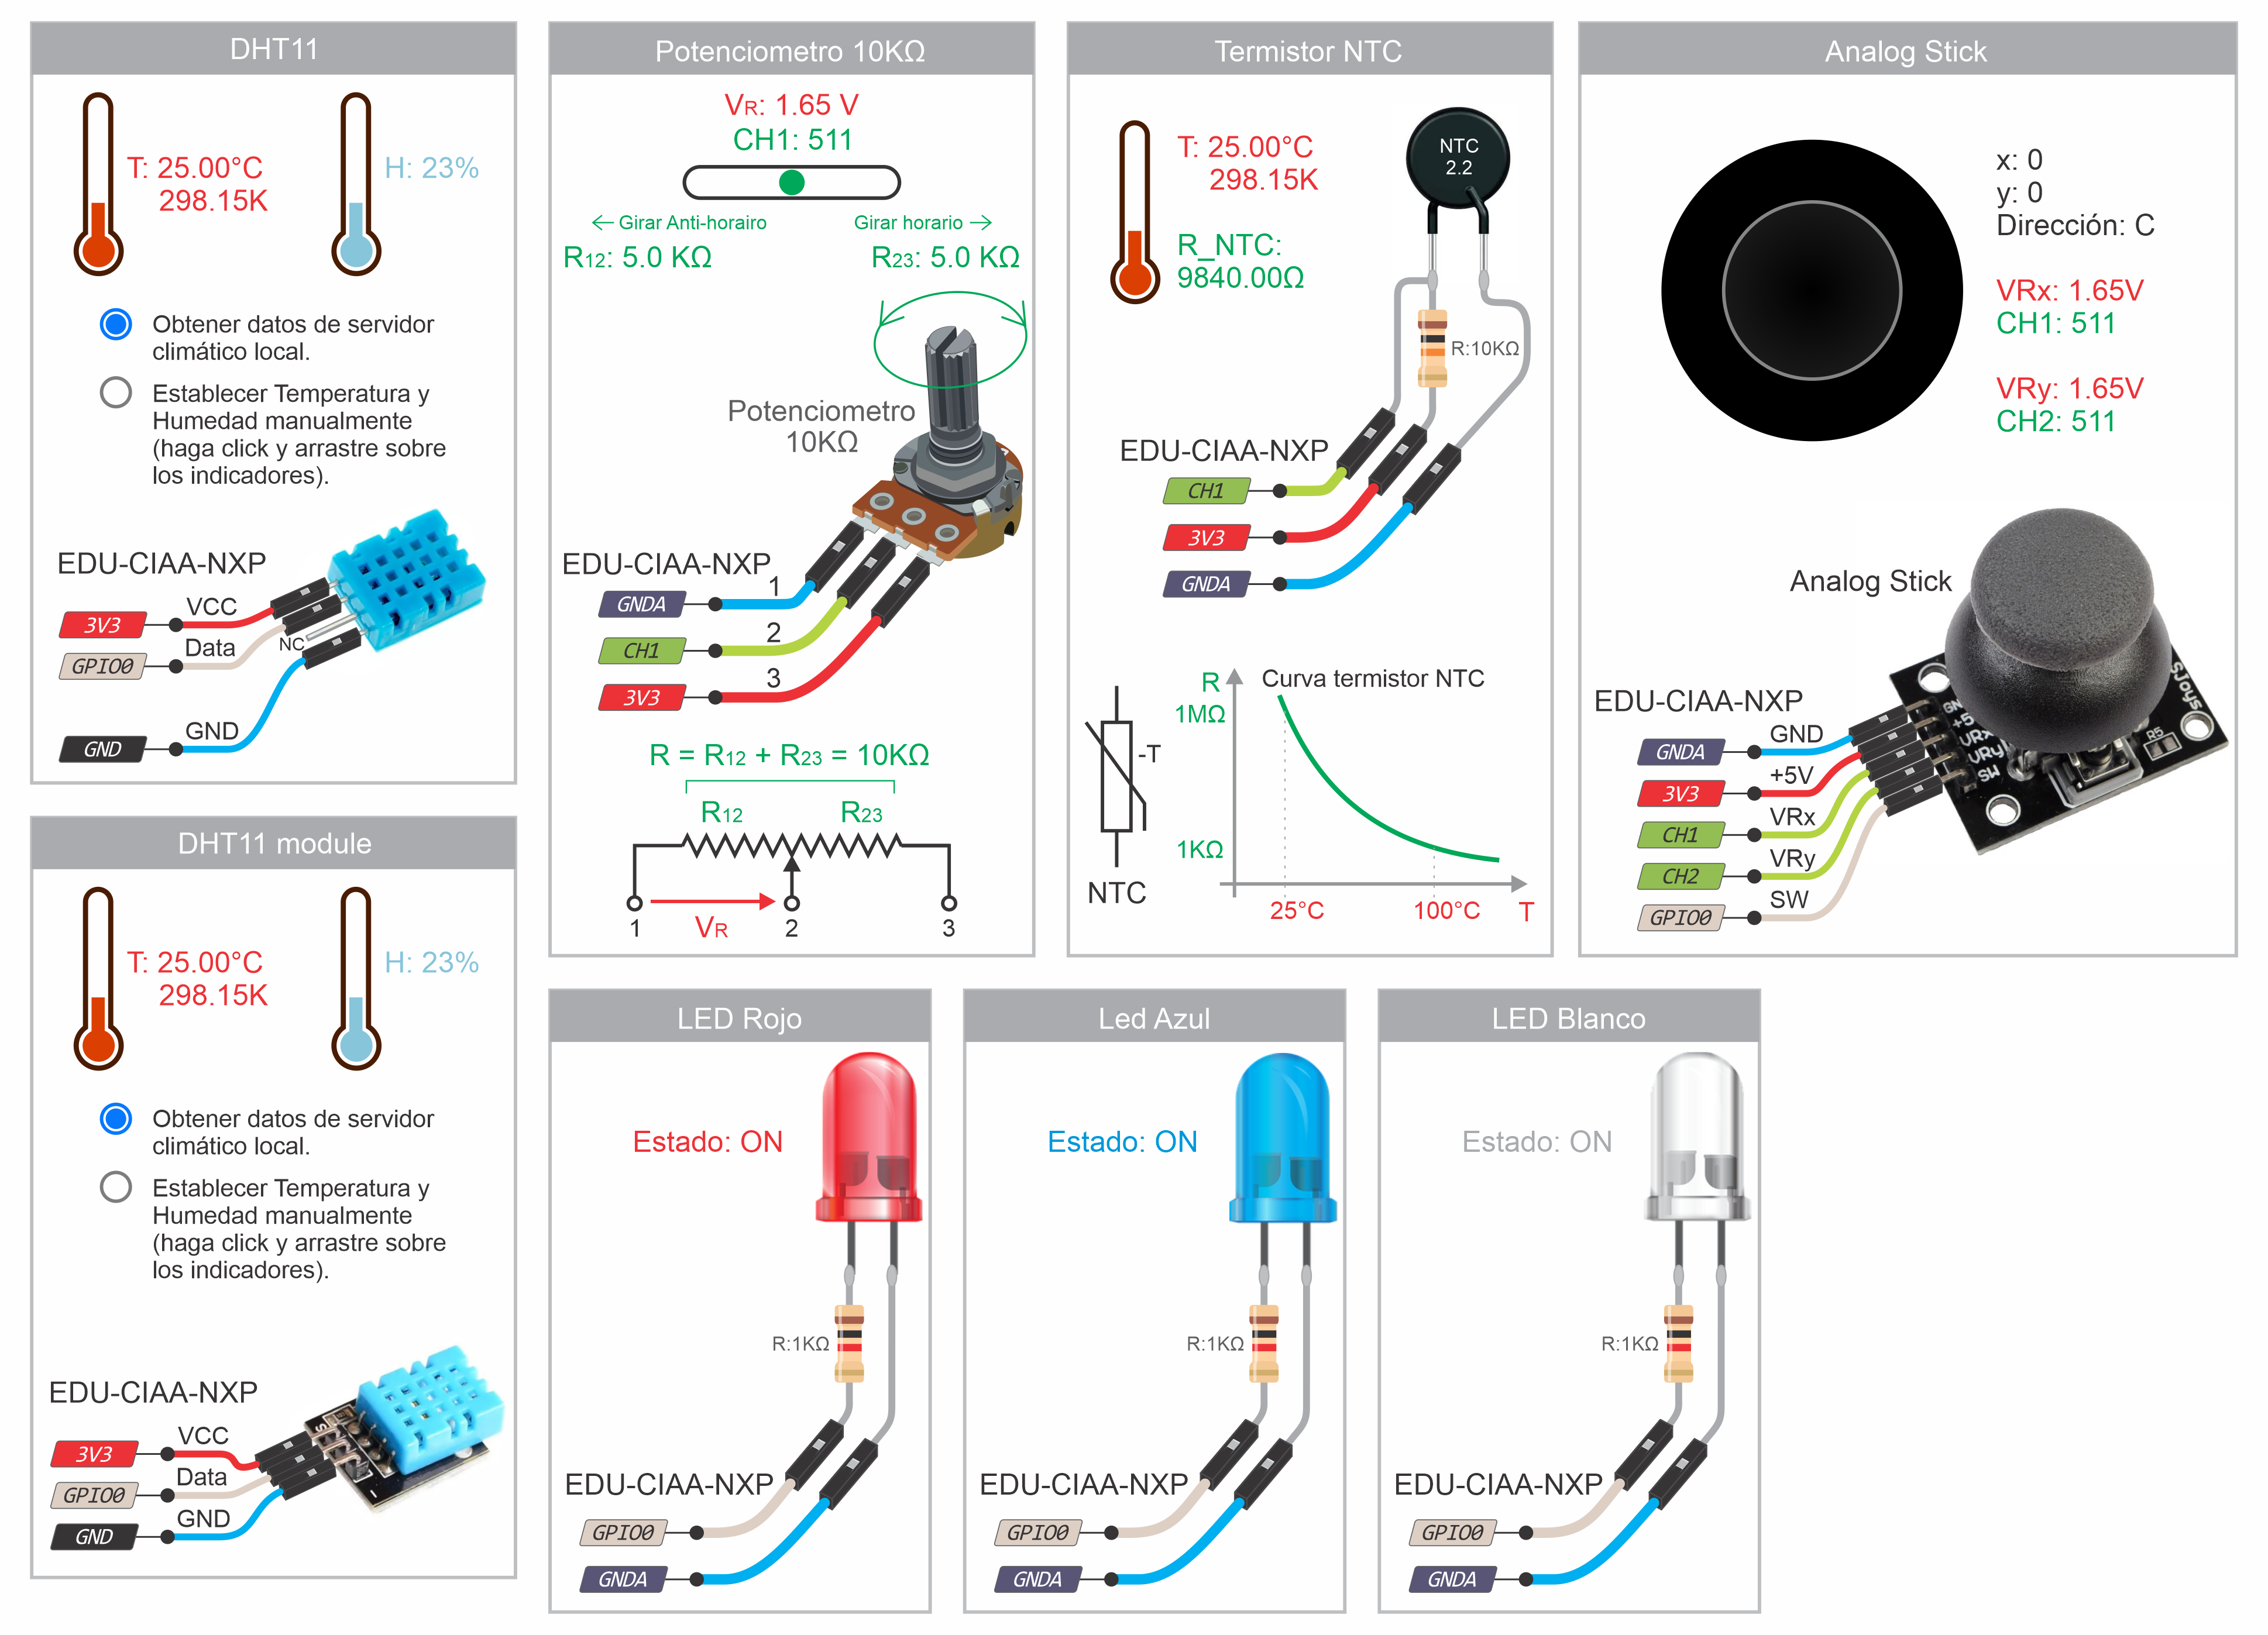
\includegraphics[scale=.40]{./Figures/perifericosCIAA.png}
	\caption{Periféricos externos del emulador web EDU-CIAA.}
	\label{fig:perifericosCIAA}
\end{figure}


\hfill \break
\hfill \break
\hfill \break
\hfill \break
\hfill \break
\hfill \break
\hfill \break
\hfill \break

\section{Caso de estudio}
\label{sec:caso_de_estudio}

El usuario escribe o modifica el programa llamado \texttt{blinky} en lenguaje \textit{C}, que utiliza la biblioteca \textit{\textbf{sAPI}} para interactuar con los periféricos de hardware GPIO y controlar el LED. A continuación, ejecuta el programa dentro de la plataforma web. Para lograr esto, Node.js se encarga de ejecutar los comandos necesarios para que \textit{Emscripten} realice la compilación del código \textit{C}, que incluye: 

\begin{itemize}
	\item El codigo de la aplicacion de usuario escrito en lenguaje \textit{C}.
	\item El archivo \texttt{sapi\_gpio.c} de la capa \textit{Bibioteca C}.
	\item El archivo \texttt{gpio\_api.c} de la capa \textit{C HAL}.
\end{itemize} 

El proceso de compilación comienza con el preprocesamiento del código \textit{C}, que incluye el manejo de directivas del preprocesador como \texttt{\#include} y \texttt{\#define}. Luego, el compilador utiliza \textit{LLVM} para compilar el código \textit{C} en \texttt{bitcode}. Después, de obtener el \texttt{bitcode} realiza optimizaciones para mejorar el rendimiento y reducir el tamaño del código resultante. Finalmente, \textit{Emscripten} toma el bitcode optimizado y lo traduce a código \textit{JavaScript}, lo que permite que el programa escrito originalmente en \textit{C} pueda ser ejecutado dentro del entorno web. Los archivos resultantes de este proceso incluyen: 


\begin{itemize}
	\item \texttt{user\_tiempoenmilisegundos.js}.
	\item \texttt{user\_tiempoenmilisegundos.wasm}.
	\item \texttt{user\_tiempoenmilisegundos.wast}.
	\item \texttt{user\_tiempoenmilisegundos.js.components}.
	\item \texttt{user\_tiempoenmilisegundos.wasm.map}.
\end{itemize}

Una vez que los archivos \texttt{.js} y \texttt{.wasm} se han generado a partir del código \textit{C}  mediante \textit{Emscripten}, pueden interactuar con el código \textit{JavaScript} de las capas: \textit{JavaScript HAL} y \textit{JavaScript UI}. Ahora bien, desde estos archivos \textit{JavaScript} de la \textit{HAL} y \textit{UI}, se pueden invocar directamente las funciones \textit{C} compiladas como si fueran funciones \textit{JavaScript} regulares, y podrán ser ejecutadas en el entorno del navegador. Por lo tanto, esto permite que el programa \textit{C} interactúe con el resto del código \textit{JavaScript} de la aplicación web y que las funciones \textit{C} puedan ser utilizadas y llamadas de manera transparente en el navegador.


La figura \ref{fig:DiagramaSecuencia} muestra la interacción del usuario con el sistema y el orden en que se producen. Además, se muestra los mensajes que se pasan entre las dependencias.
\hfill \break
\hfill \break
\hfill \break
\hfill \break
\hfill \break
\hfill \break
\hfill \break
\hfill \break
\hfill \break
\hfill \break

\begin{figure}[ht]
	\centering
	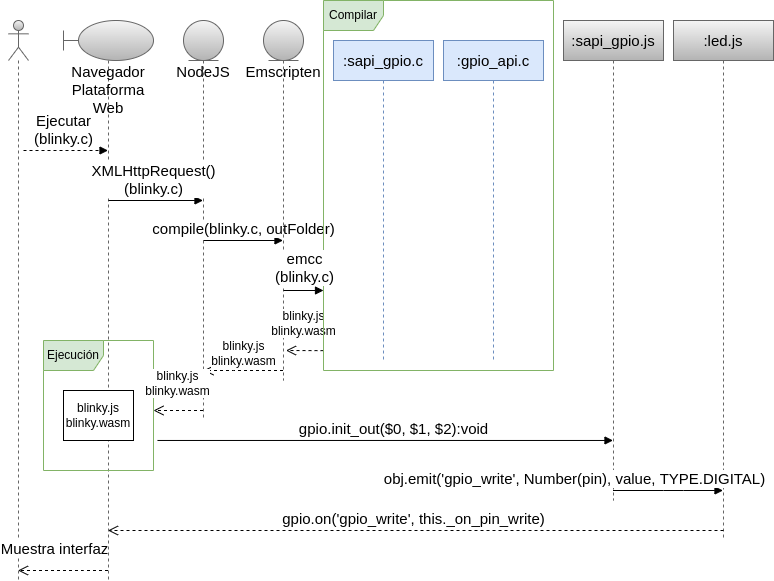
\includegraphics[scale=.49]{./Figures/DiagramaSecuencia.png}
	\caption{Interacción del usuario con las dependencias del emulador.}
	\label{fig:DiagramaSecuencia}
\end{figure}

Además, la capa \textit{JavaScript HAL}, que interactúa con el código \textit{JavaScript} resultante de la compilación de la \textit{Biblioteca C} y \textit{C HAL}, se encarga de notificar los eventos ocurridos en esas capas para el programa de usuario \texttt{blinky}. Mediante la función \texttt{write}, se realiza la activación del evento que escribe en la GPIO, Como resultado, emitirá el evento con el nombre \texttt{gpio\_write}, pasando como argumentos el número de pin, el valor digital y el tipo de pin declarado.


La figura \ref{fig:GPIOEventEmitter} muestra el diagrama en bloques del evento con el nombre \newline \texttt{gpio\_write}.

\begin{figure}[ht]
	\centering
	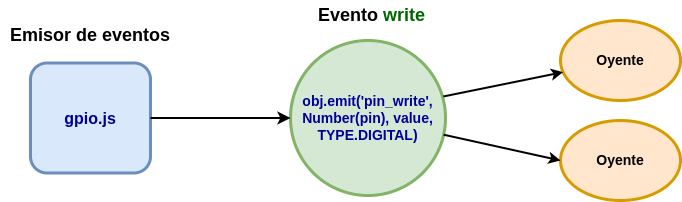
\includegraphics[scale=.40]{./Figures/GPIOEventEmitter.png}
	\caption{Activación de evento con el nombre \texttt{gpio\_write}.}
	\label{fig:GPIOEventEmitter}
\end{figure}



En ese sentido, en la capa \textit{JavaScript UI}  cuando se emite el evento con el nombre \texttt{gpio\_write}, cualquier oyente que esté suscrito a ese evento podrá escucharlo y realizar las acciones correspondientes para la funcionalidad que se requiere. En este caso, la acción solicitada es encender el LED.

La figura \ref{fig:ListeningGPIOEventEmitter} muestra el diagrama en bloques del oyente subscrito al evento \texttt{gpio\_write}.


\begin{figure}[ht]
	\centering
	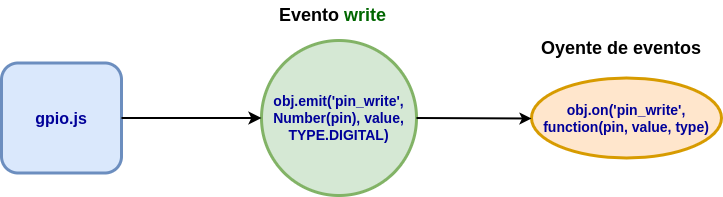
\includegraphics[scale=.40]{./Figures/ListeningGPIOEventEmitter.png}
	\caption{GPIO oyente del evento con el nombre \texttt{gpio\_write}.}
	\label{fig:ListeningGPIOEventEmitter}
\end{figure}

Entonces, en la plataforma web se muestrarán los cambios de \texttt{gpio\_write} en la placa virtual. 

En la figura \ref{fig:AplicacionUsuarioLeds} se presenta para una función de la GPIO, la interacción entre todas las capas de programación.


\begin{figure}[ht]
	\centering
	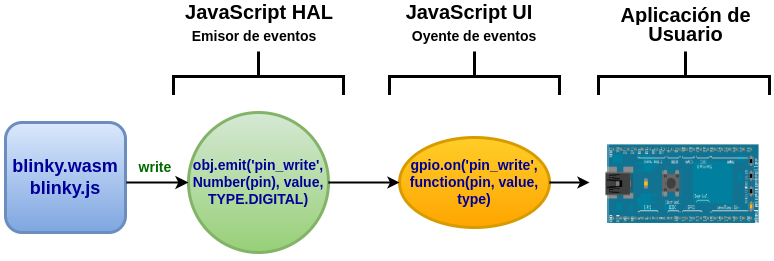
\includegraphics[scale=.36]{./Figures/AplicacionUsuarioLeds.png}
	\caption{Interacción entre todas las capas de programación.}
	\label{fig:AplicacionUsuarioLeds}
\end{figure}


\section{Despliegue}


Para hacer público el emulador de la plataforma en un servidor web, se realizó el proceso de despliegue en el servidor de \textit{DigitalOcean} mediante los siguientes pasos:


\begin{itemize}
	\item Crear una cuenta: implicó registrar una cuenta en la plataforma. Después de iniciar sesión, se creo un \textit{droplet}, que es un servidor virtual. Luego, se instaló el sistema operativo \textit{Ubuntu}, y se configuró la región geográfica donde se ubicaría el servidor y la cantidad de RAM.
	
	\item Acceso al servidor: después que el \textit{droplet} fue creado, se pudo  obtener la dirección IP pública y la clave \textit{SSH} para acceder al servidor.
	
	\item Configuración: implicó instalar las herramientas, como \textit{Mbed CLI} y \textit{Emscripten}, y también, los servicios necesarios, como los entornos de ejecución de \textit{Node.js} y \textit{Python}. Además, se realizó las configuraciones de las reglas de \textit{firewall}.

	\item Copiar la plataforma web al servidor: se utilizó \textit{GitHub}  para clonar el repositorio en el servidor. El código del presente trabajo, se encuentra en el repositorio de GitHub \citep{repositorioEmulador}.
	
	\item Iniciar el emulador web: se utilizó la herramienta \textit{TMUX} para mantener la sesión y la ventana de la terminal donde se ejecuta la aplicación de forma persistente, incluso cuando se cierra la conexión  \textit{SSH}. El presente trabajo, se encuentra actualmente ejecutandose en 
\url{http://134.209.168.175:7900}.
\end{itemize}





